
% ============================================================
%  ModuCard System 3 — Handbook
% ============================================================
\documentclass[b5paper, 10pt, twoside]{book}

\usepackage[T1]{fontenc}
\usepackage[utf8]{inputenc}

% ── Fonts ───────────────────────────────────────────────────
% Body: Palatino (warm, slightly old-school)
% Titles: Helvetica bold condensed (TI-style authority)
\usepackage{palatino}
\usepackage[scaled=0.92]{helvet}
\usepackage{courier}

% ── Geometry ────────────────────────────────────────────────
\usepackage[
  b5paper,
  top=20mm, bottom=24mm,
  inner=22mm, outer=18mm,
  headheight=13pt
]{geometry}
\usepackage{tabularx}
\usepackage{float}

% ── Colors ──────────────────────────────────────────────────
\usepackage{xcolor}
\definecolor{inkBlack}{RGB}{18, 16, 14}      % warm near-black (not cold)
\definecolor{paperCream}{RGB}{250, 246, 235} % aged paper
\definecolor{accentRed}{RGB}{185, 40, 30}    % TI-style accent
\definecolor{midGray}{RGB}{130, 125, 118}
\definecolor{lightGray}{RGB}{210, 205, 195}

% ── TikZ ────────────────────────────────────────────────────
\usepackage{tikz}
\usetikzlibrary{calc, decorations.pathmorphing, decorations.markings}

% Hand-drawn line style — slight wobble
\tikzset{
  hand/.style={
    decorate,
    decoration={random steps, segment length=4pt, amplitude=0.4pt},
    line cap=round, line join=round
  },
  handthick/.style={
    decorate,
    decoration={random steps, segment length=5pt, amplitude=0.5pt},
    line width=2.2pt, line cap=round, line join=round
  },
  handfill/.style={
    decorate,
    decoration={random steps, segment length=3pt, amplitude=0.3pt},
    line cap=round, line join=round, fill
  }
}

% ── Microtype & layout ──────────────────────────────────────
\usepackage{microtype}
\usepackage{ragged2e}
\usepackage{multicol}
\usepackage{setspace}

% ── Headers ─────────────────────────────────────────────────
\usepackage{fancyhdr}
\pagestyle{fancy}
\fancyhf{}
\fancyhead[LE]{\small\sffamily\textbf{ModuCard System 3}}
\fancyhead[RO]{\small\sffamily\textbf{\leftmark}}
\fancyfoot[C]{\small\sffamily\thepage}
\renewcommand{\headrulewidth}{0.5pt}

% ── Chapter / section titles ────────────────────────────────
\usepackage{titlesec}

% Chapter: big slab number + hand-rule underneath
\titleformat{\chapter}[hang]
  {\sffamily\bfseries\LARGE}
  {\thechapter}{1em}{}[\vspace{4pt}\titlerule]
\titlespacing*{\chapter}{0pt}{*2}{*2}

\titleformat{\section}
  {\sffamily\bfseries\normalsize}
  {\thesection}{1em}{}[{\color{inkBlack}\rule{\linewidth}{0.3pt}}]
\titlespacing*{\section}{0pt}{*1.5}{*0.8}

\titleformat{\subsection}
  {\sffamily\bfseries\small}
  {\thesubsection}{1em}{}
\titlespacing*{\subsection}{0pt}{*1}{*0.5}

% ── Utilities ───────────────────────────────────────────────
\usepackage{booktabs}
\usepackage{enumitem}
\usepackage{siunitx}
\usepackage{listings}
\usepackage{hyperref}
\hypersetup{hidelinks}

\lstset{
  basicstyle=\footnotesize\ttfamily,
  backgroundcolor=\color{lightGray!30},
  frame=single, framerule=0.4pt,
  rulecolor=\color{midGray},
  numbers=left, numberstyle=\tiny\color{midGray},
  breaklines=true
}

% ── Note box (hand-border style) ────────────────────────────
\newcommand{\mcsbox}[2][Note]{%
  \vspace{6pt}%
  \noindent
  \begin{tikzpicture}
    \node[inner sep=7pt, text width=\dimexpr\linewidth-14pt] (txt)
      {\footnotesize\rmfamily\textbf{#1:} #2};
    \draw[hand, line width=1pt, inkBlack]
      (txt.north west) rectangle (txt.south east);
  \end{tikzpicture}%
  \vspace{4pt}%
}

\newcommand{\mcs}{\textsf{\textbf{MCS\,3}}}
\newcommand{\mcsfull}{ModuCard System~3}


% ============================================================
\begin{document}
% ============================================================

% ────────────────────────────────────────────────────────────
%  COVER — full page photo only
% ────────────────────────────────────────────────────────────
\begin{titlepage}
  \newgeometry{margin=0pt}
  \thispagestyle{empty}
  \noindent
  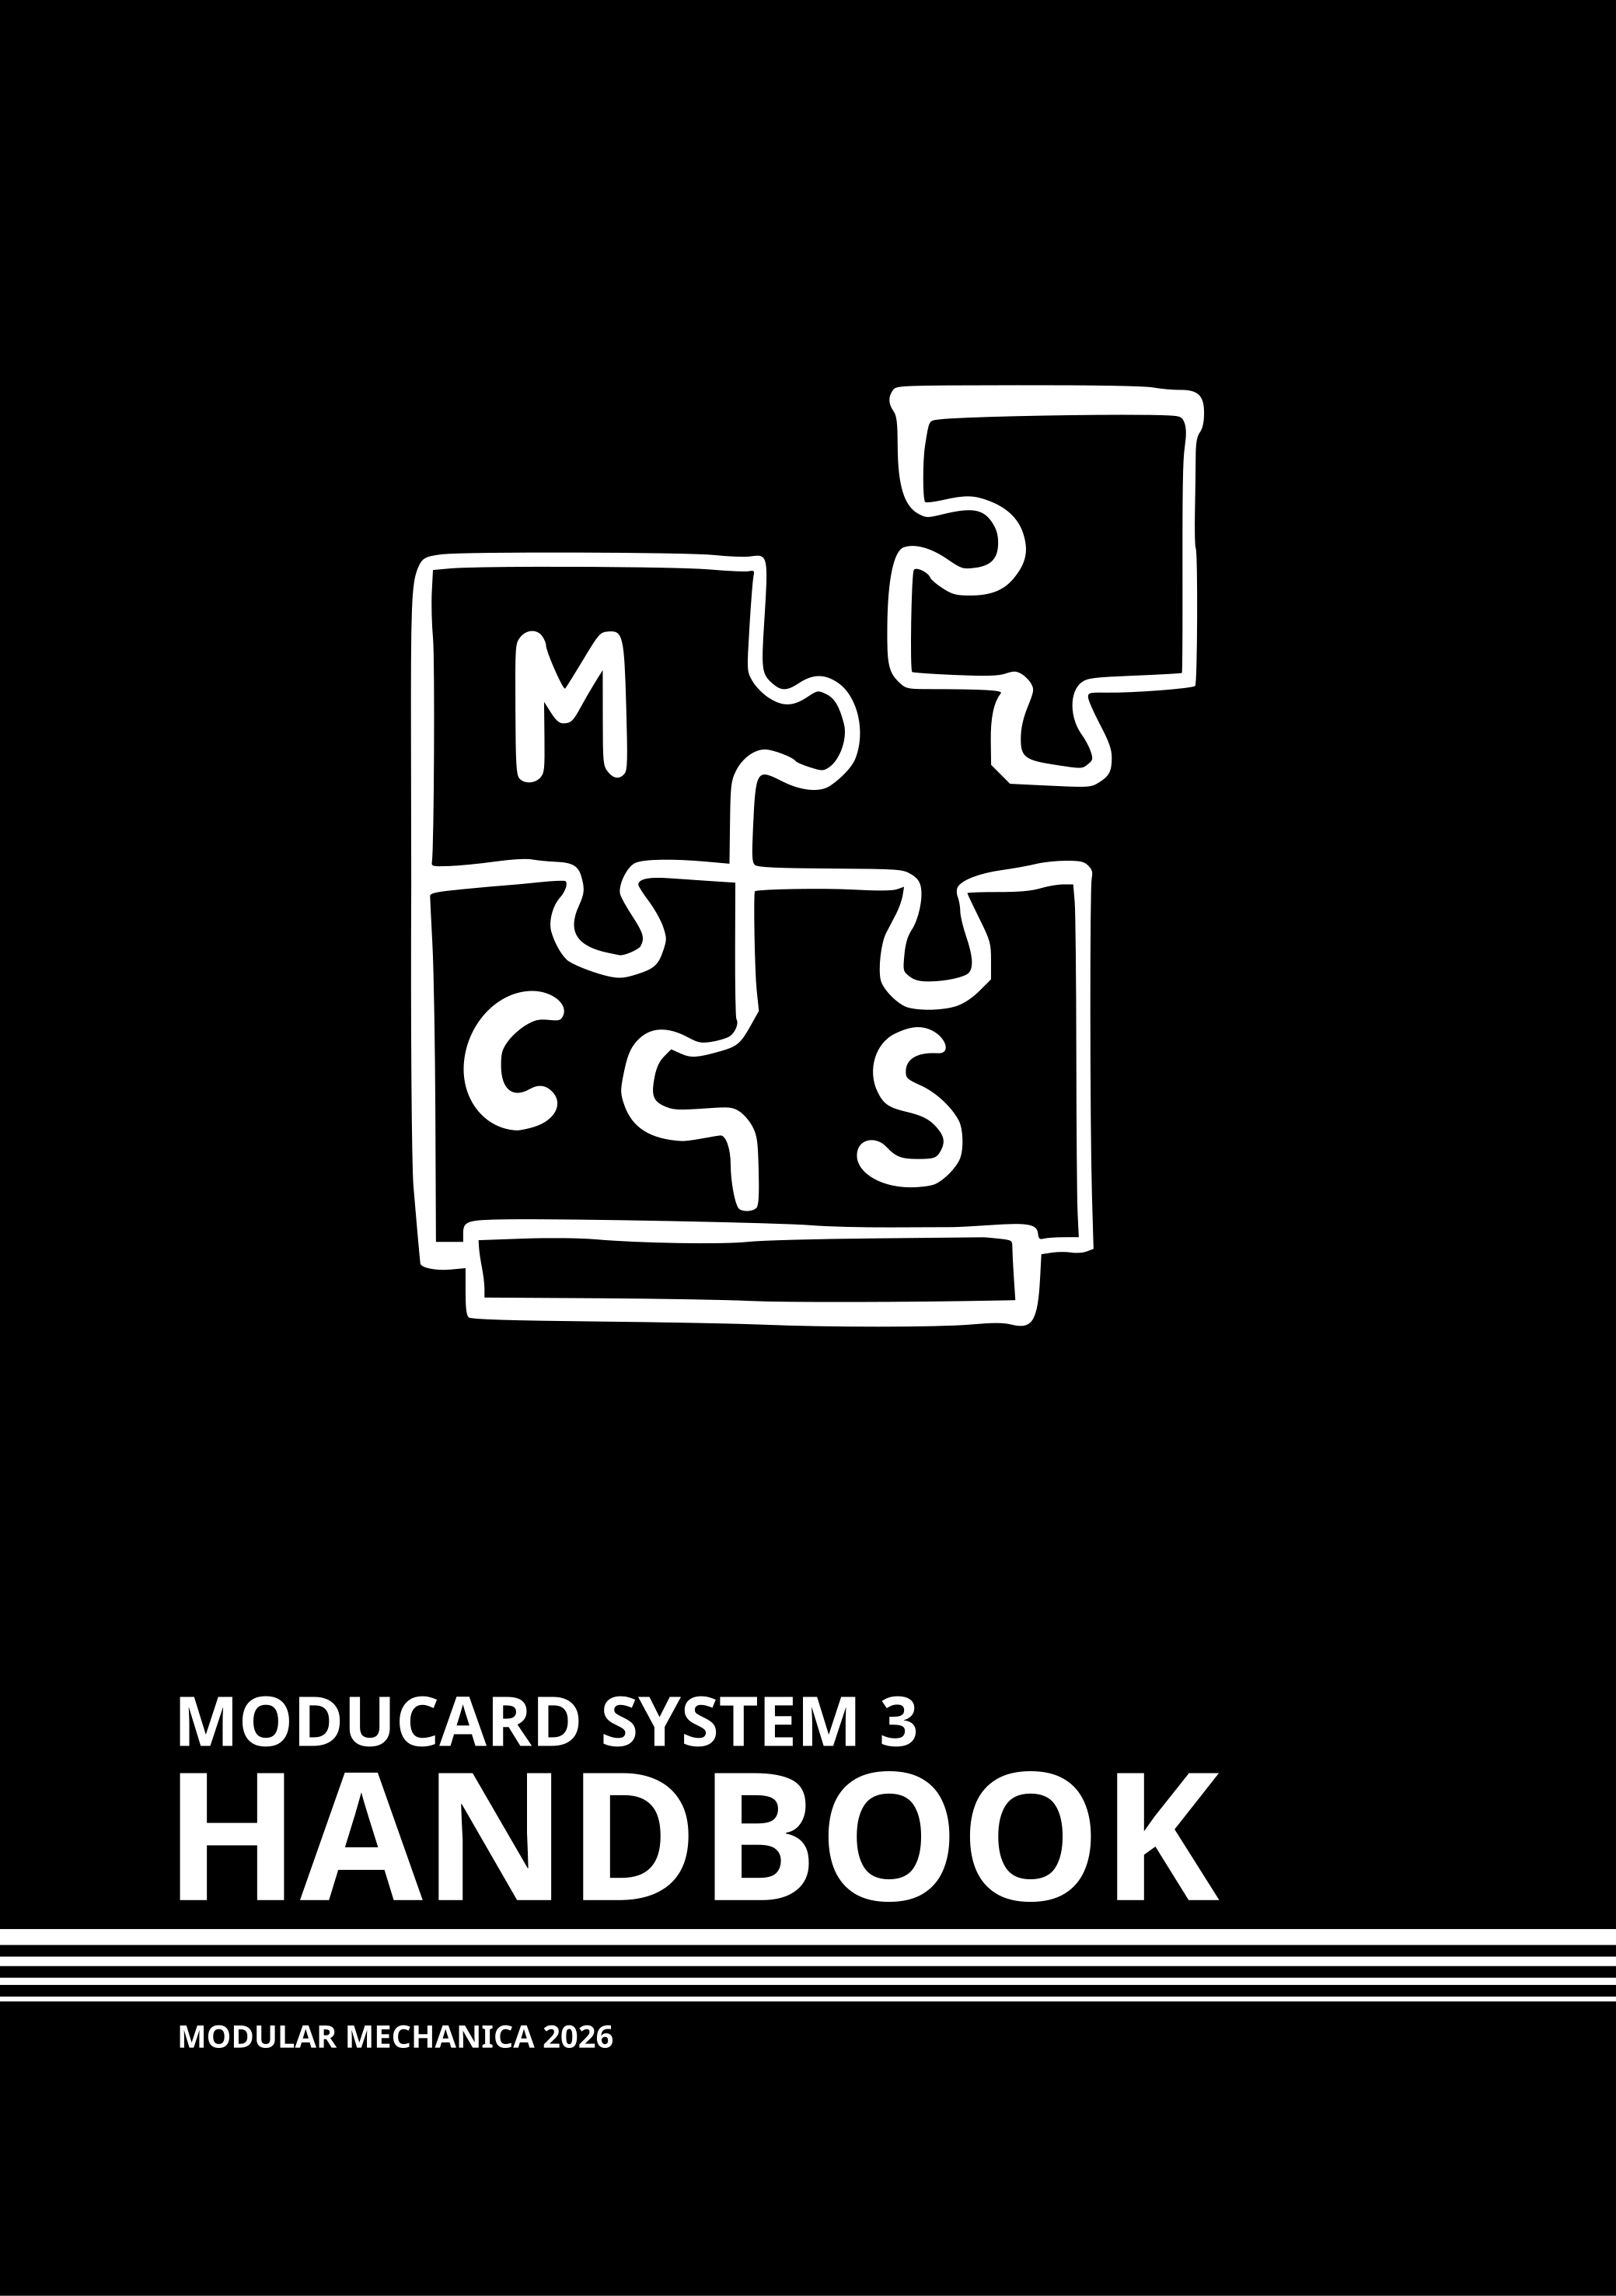
\includegraphics[width=\paperwidth,height=\paperheight,keepaspectratio=false]{photos/ModuCard-Handbook.png}
  \restoregeometry
\end{titlepage}

% ────────────────────────────────────────────────────────────
%  VERSO — title page (TI inner style, warm paper)
% ────────────────────────────────────────────────────────────
\thispagestyle{empty}
\color{inkBlack}

\vspace*{10mm}

{\sffamily\fontsize{8}{9}\selectfont\bfseries
  \MakeUppercase{MODULAR MECHANICA 2026}}\par
\vspace{14mm}

\noindent\rule{\linewidth}{0.3pt}\par
\vspace{8mm}
% Inner title — mirrors TI-82 exactly
{\sffamily\fontsize{40}{40}\bfseries\selectfont MCS\,3}\par
\vspace{2mm}
{\sffamily\fontsize{9}{10}\bfseries\selectfont
  \MakeUppercase{ModuCard System}}\par
\vspace{2mm}
{\sffamily\fontsize{20}{20}\bfseries\selectfont
  \MakeUppercase{Handbook}}\par


{\small\rmfamily
  \vfill
  \vspace{3mm}
  {\footnotesize\rmfamily
    Copyright \textcopyright\ 2024 by Modular Card Consortium.
    All rights reserved.\par
    \vspace{2mm}
    \textit{Modular Card System} and \textit{MCS} are trademarks of the
    Modular Card Consortium. All other trademarks belong to their
    respective owners.
  }
}

\clearpage
\pagecolor{white}
\color{black}


% ────────────────────────────────────────────────────────────
%  FRONT MATTER
% ────────────────────────────────────────────────────────────
\frontmatter
\pagestyle{fancy}
\tableofcontents
\clearpage


% ────────────────────────────────────────────────────────────
%  CHAPTER 1 — INTRODUCTION
% ────────────────────────────────────────────────────────────
\mainmatter

\chapter{Fork}
\section{Dlaczego tak chaotycznie}
ogólnie potrzebuję pisać i mieć gdzie pokazać nowym ludziom jak to działa.
Jeśli będą rzeczy w różnych językach, pomieszane, powtórzone itd to sorka.
Potrzeba żeby ktoś napisał jak to działa faktycznie, zrobił zdjęcia
a potem się to rzuci do Chata "popraw to. make no mistake".

\section{Sekcje}
Wstępnie planowaliśmy podzielić handbooka na kilka książek, jedna dla elektronika
jedna dla programisty etc. Ale mi się będzie łatwiej pisało w jednym pliku, więc here
we are.

\section{Prezentacja}
Kiedyś zrobiłem prezentację o ModuCardzie. Przerzucam wszystko co ważne w niej tutaj,
w szczególności to co techniczne. Jeśli jej szukasz, to wszystko jest w tej książce
jak na razie.


\section{Język}
Spoko byłoby pisać dokumentację po angielsku, bo to poważny system a angielski to poważny język.
Maybe another day.

\section{Struktura}
Zacznij czytać od Primera, tam jest ogólny opis systemu. W rozdziałach ModuCard - zasada działania
masz trochę więcej szczegółów, a potem w kolejnych rozdziałach masz już wszystkie szczegóły.
Znowu to samo powtarzam w rozdziałach projektowanie kart/hatów. Jak nie załapiesz, to zapytaj się kogoś z koła.

\section{I reszta}

Aktualnie książka jest do użytku wewnętrznego KoNaR-u, ale możecie na spokojnie
ją udostępniać komu trzeba. Czasem będę rzucał inside joke'i albo nazwiskami jak coś.

Fork jest mój, Wojtka Szafrańskiego (@themuse061 na Discordzie), a siedzę głównie w elektronice. Ona będzie
najdokładniej opisana, mechanika też git powinna być, ale programowanie będzie tak sobie.

\textbf{Oh, i możesz szukać "Jak projektować hat'a \ref{MiniModuCard - Projektowanie hatów}"
  albo "jak projektować Karte \ref{Duży ModuCard - Projektowanie kart}"}

% \chapter{Introduction}

% \section{About This Handbook}

% This handbook describes the \mcsfull\ (\mcs) interface standard —
% a system of interlocking modular robotic cards that can be freely
% combined, extended, and reconfigured without tools.

% \mcsbox{Read this chapter in full before assembling any modules.
%   Incorrect insertion order may damage bus termination circuits.}

% The document is structured in four self-contained parts. Each part
% can be read independently; cross-references indicate dependencies
% where they exist.

% \section{What Is \mcsfull?}

% \mcs\ is a family of interchangeable robotic building blocks.
% Every module exposes four standardised connector faces
% (N, S, E, W) and communicates over a shared differential bus.
% Modules are hot-swappable: the bus protocol detects insertion
% and negotiates addresses automatically.

% \medskip
% \noindent Core properties at a glance:

% \begin{itemize}[itemsep=3pt, topsep=4pt, leftmargin=*]
%   \item \textbf{Power:} \SI{24}{\volt} shared rail,
%         \SI{3}{\ampere} per face maximum
%   \item \textbf{Data:} \SI{10}{\mega bit\per\second}
%         half-duplex serial, CRC-16 framing
%   \item \textbf{Addressing:} automatic negotiation on hot-attach
%   \item \textbf{Topology:} tree or daisy-chain, up to 63 modules
% \end{itemize}

% \section{Conventions Used in This Handbook}

% \begin{description}[style=nextline, leftmargin=10mm,
%     itemsep=4pt, topsep=4pt]
%   \item[\texttt{Monospace}]
%         Register names, bus commands, and literal byte values.
%   \item[\textbf{Bold sans}]
%         First use of a defined term; see Glossary (Appendix~A).
%   \item[{[ranges]}]
%         Square brackets denote inclusive value ranges,
%         e.g.\ \texttt{[0x00--0xFF]}.
%   \item[Dimensions]
%         All dimensions in millimetres at \SI{20}{\degreeCelsius}
%         unless otherwise stated.
% \end{description}

% \mcsbox[Important]{Chapters marked $\star$ in the Table of Contents
%   contain normative requirements (shall / shall not).
%   All other chapters are informative.}

% \section{How To Use This Handbook}

% If you are a \textbf{hardware designer}, start with Part~I
% (Mechanical) and Part~II (Electrical), then refer to Part~IV
% (Conformance) for test procedures.

% If you are a \textbf{firmware developer}, start with Part~III
% (Communication Protocol), where the complete packet format and
% API are defined.

% If you are a \textbf{system integrator}, Part~I Chapter~3
% (Assembly Rules) and Part~III Chapter~9 (Topology Planning)
% are the most immediately useful sections.

\chapter{Primer -> Zacznij tutaj} \label{Primer}
\section{Co i po co - Część \#1 "Co"}
ModuCard to system dwóch standardów do tworzenia projektów robotycznych. Można w nim zrobić roboty, które wykonują
skomplikowane czynności (chodzenie, regulacja procesów technologicznych, wizja komputerowa i inne).

Jest wymyślony w taki sposób, żeby zminimalizować ilość pracy włożoną w projektowanie i
naprawianie robotów. Realizowane jest to przez używanie takich samych elementów w wielu miejscach.
Te elementy są zgodne ze standardem, więc łatwo \textbf{je} zaprojektować oraz łatwo \textbf{do nich}
zaprojektować mechanikę i programowanie. Czytaj: co tylko się da, ma takie same wymiary i złącza.

\subsection{Duży ModuCard a MiniModuCard}
\begin{itemize}
  \item ModuCard (nazywany też dużym ModuCardem) -> Duże karty wpinane do backplate'a jak karta graficzna do płyty
        głównej. Na kartach dużego ModuCarda są bardziej wymagające peryferia, jakieś kamery, duże zasilacze, całe podsystemy.
        ModuCard to mózg całego systemu -> ma w sobie główny komputer systemu, analizuje dane, decyduje co zrobić dalej i
        steruje MiniModuCardem.
  \item MiniModuCard -> Haty wpinane do MMS-a. MMS to płytka z mikrokontrolerem i zasilaczem 5V. Na hatach są proste układy,
        które robią jedną rzecz, np. sterowniki silników, czujniki jakości powietrza, sterowniki taśm LED, przekaźniki.
        MiniModuCard to ręce i oczy systemu - wykonują pracę, raportują wartości czujników etc.
\end{itemize}


% /#\#/\/#\ Kijowa nazwa alert: MMS nazywa się tak samo jak MiniModuCard. System i jego cpu

ModuCard i MiniModuCard komunikują się ze sobą dwiema liniami CAN. Taki protokół komunikacyjny wymyślony
do samochodów. Jest spoko, bo wiesz, że jak wyślesz jakąś paczkę danych, to na pewno dojdzie do adresata, ma priorytety wiadomości i inne.
Te same linie CAN idą przez duży i mały ModuCard.

\subsection{Naprawa i wytrzymałość}

Wszystkie elementy, z których złożony jest robot w ModuCardzie, są wymienialne. Jak ci się zepsuje jakaś karta, to możesz
ją po prostu wyjąć i włożyć nową, dokładnie taką samą. Te złącza, na które się wpinają, Artem (ten, co ogólnie wymyślił ten standard)
zakosił z kolei, więc są całkiem odporne. Jak raz chłopaki
wjechali łazikiem w ścianę, to sytuacja była analogiczna do Nokii 3310 spadającej na podłogę. MiniModuCard też ma podobny wątek, fajne złącza, modularność,
łatwa wymiana i tak dalej.

\subsection{Uniwersalność}

Oh, i w ModuCardzie można nie tylko robić duże i poważne roboty. Nawet nie tylko roboty. Jak chcesz, to możesz robić
instalację produkcyjną, jak w Hefajsosie (maszyna do przerobu odpadów w filament 3D) albo wziąć tylko MiniModuCarda
i używać go jak Arduino. Wpinasz hata z przekaźnikiem, jakieś PWM-y i komunikację po UART i już możesz przełączać żarówki w smart home'ie.

I to były słowa. Co do zdjęć...
\newpage
\subsection{ModuCard zdjęcia}

\begin{figure}[!h]
  \centering
  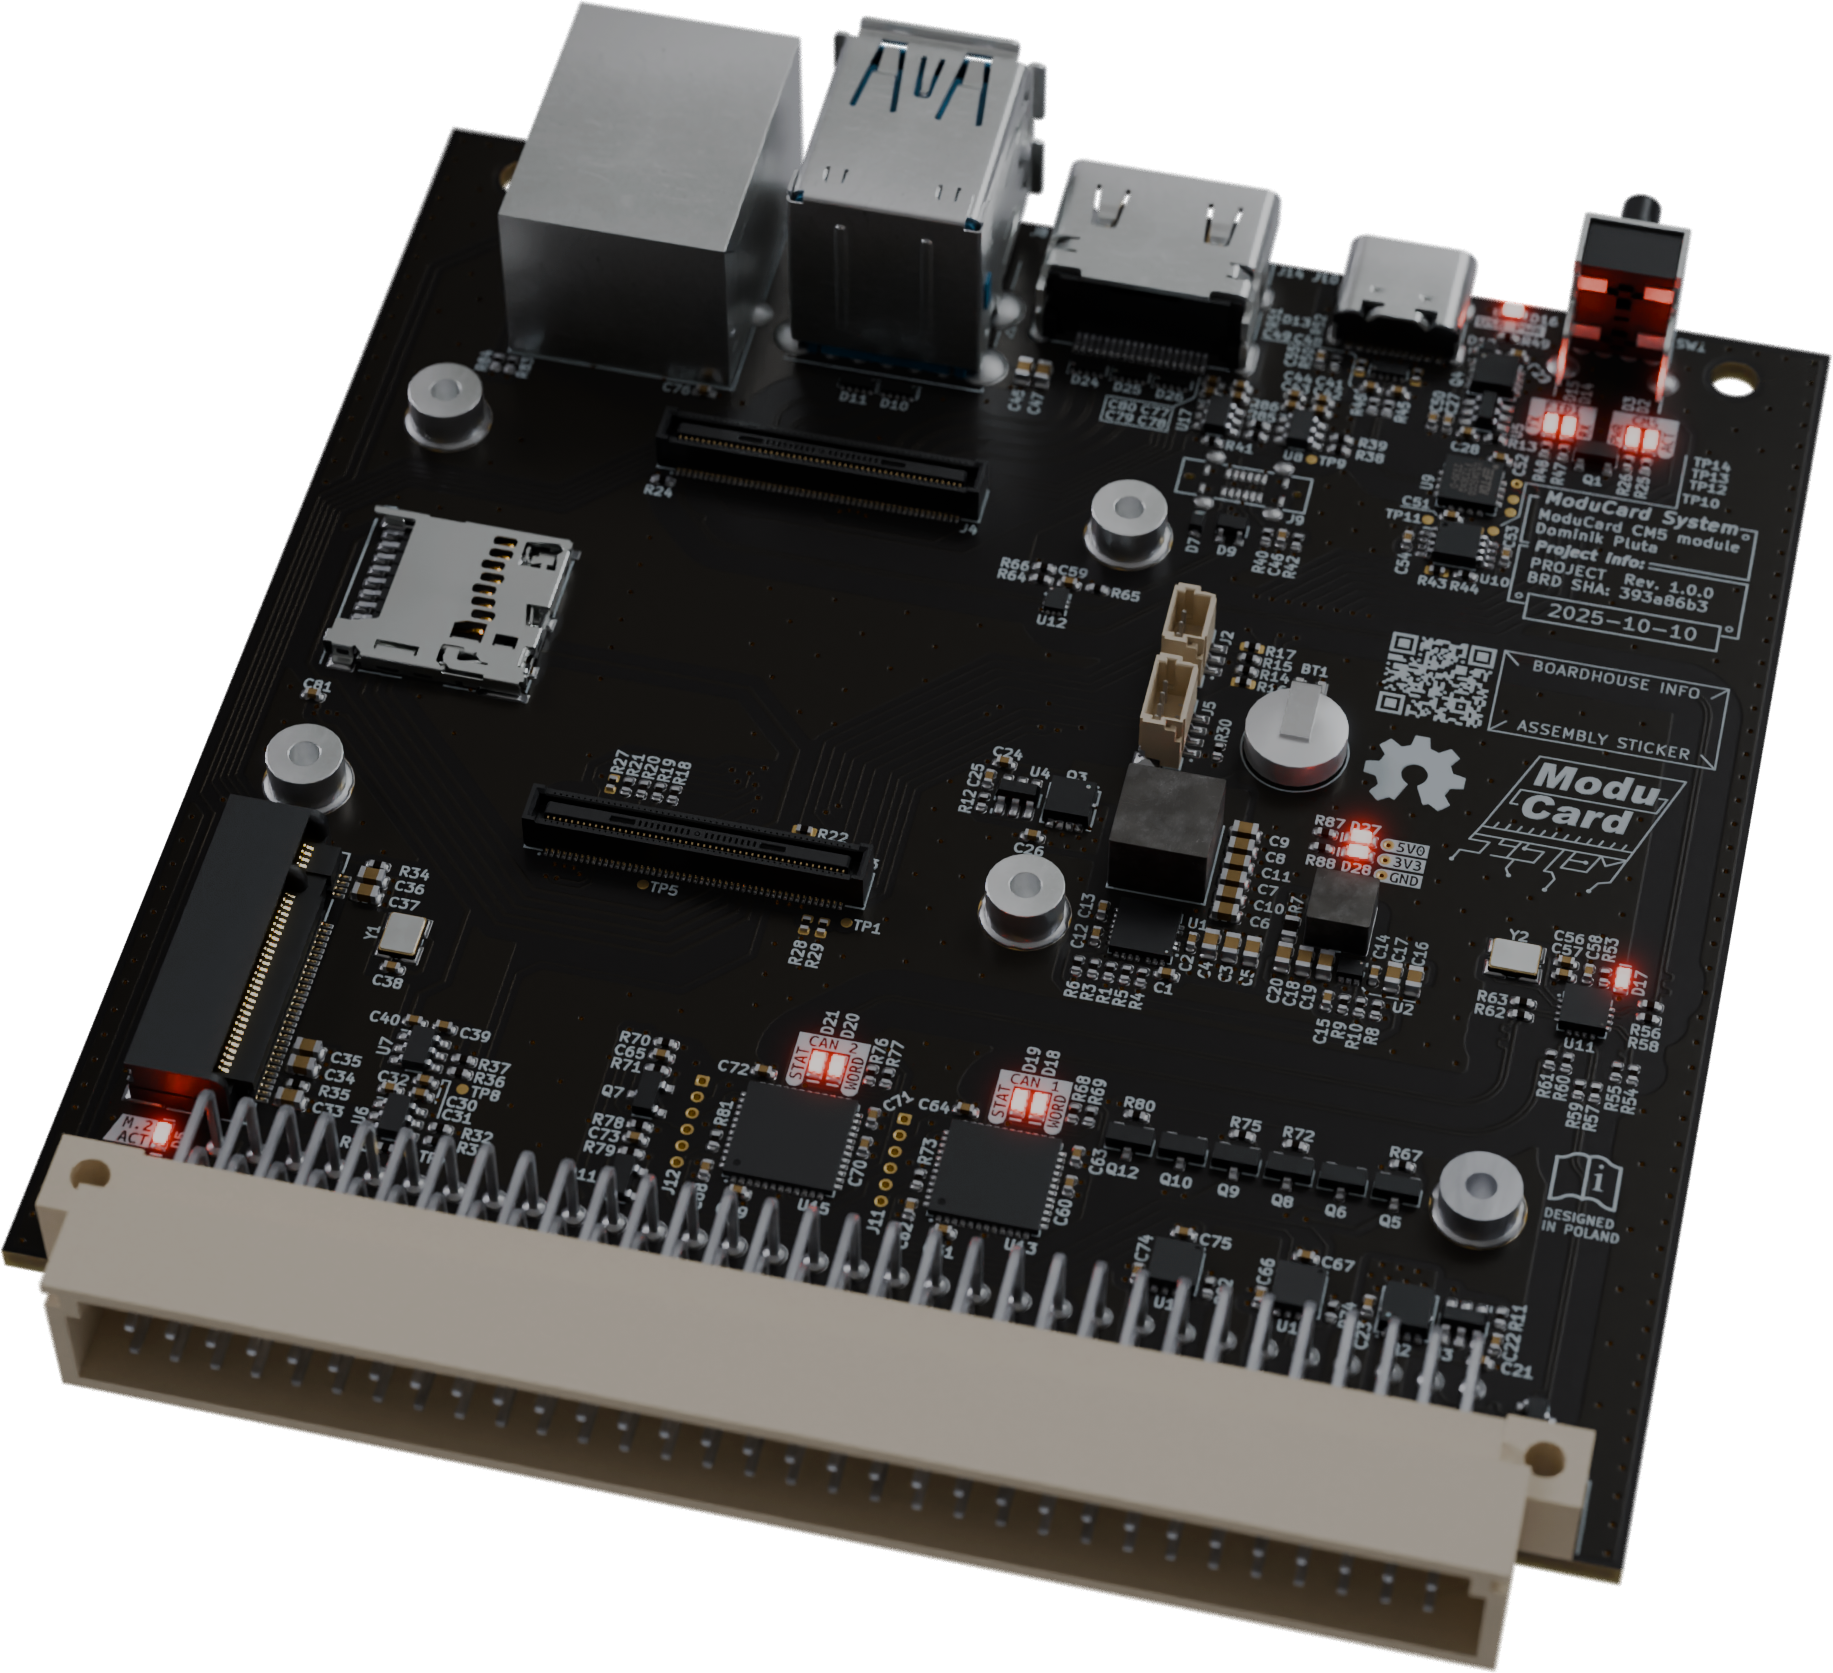
\includegraphics[width=0.5\textwidth]{photos/moducard one board.png}
  \caption{Pojedyncza karta ModuCard}
  %\label{fig:NoLabel}
\end{figure}

\begin{figure}[!h]
  \centering
  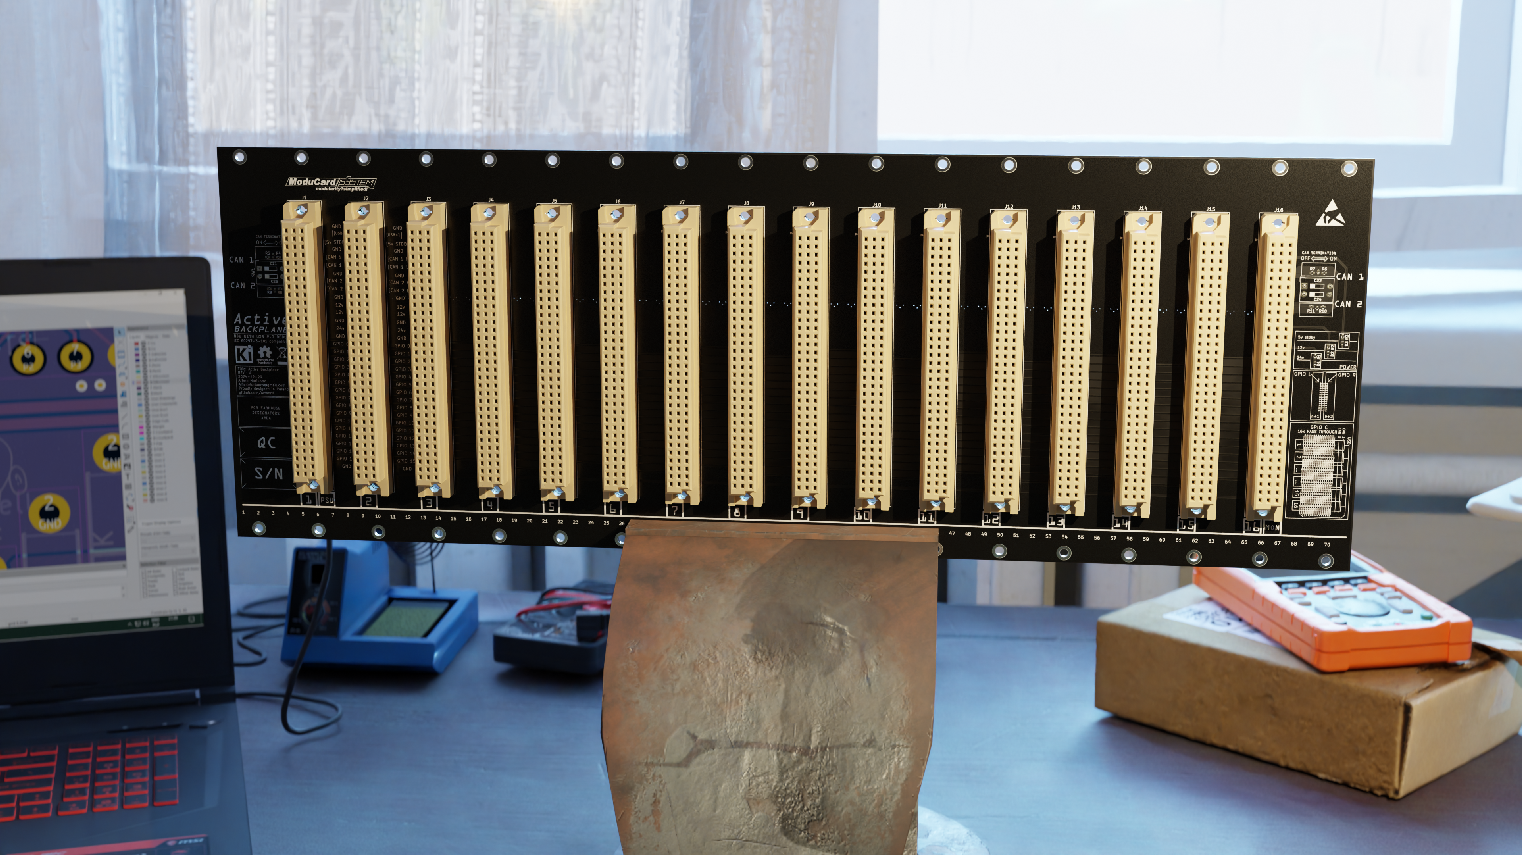
\includegraphics[width=0.5\textwidth]{photos/Moducard Backplane.png}
  \caption{Backplane ModuCard. Do niego wpina się karty}
  % \label{fig:Nomad_ModuCard}
\end{figure}

\begin{figure}[!h]
  \centering
  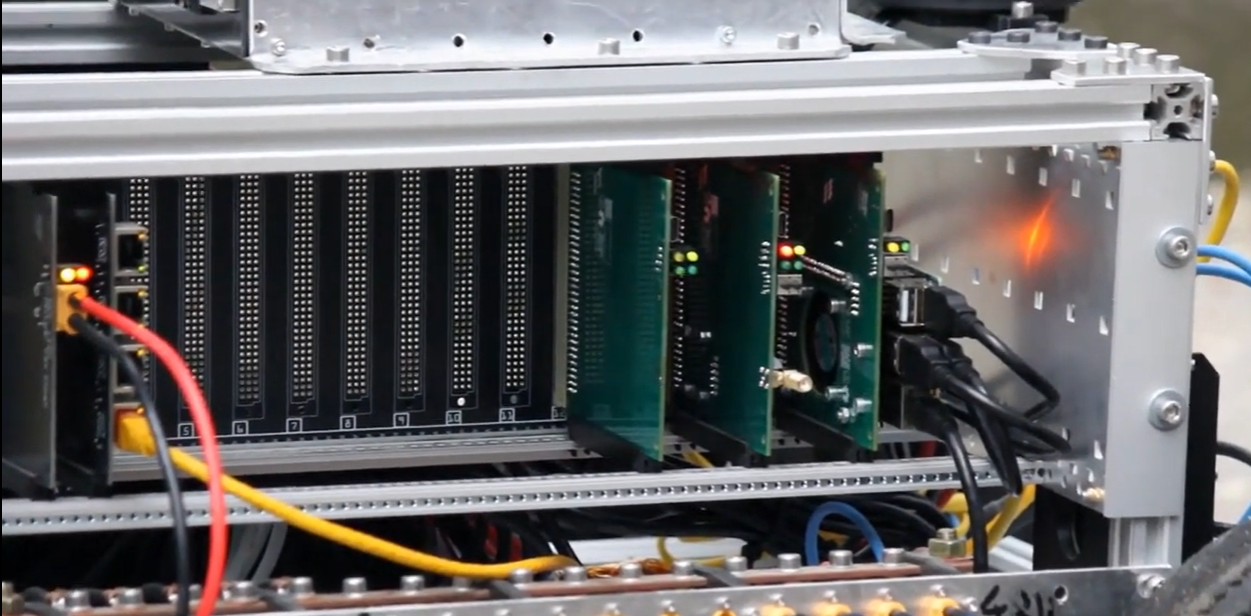
\includegraphics[width=0.7\textwidth]{photos/Nomad_ModuCard.png}
  \caption{Na zdjęciu są karty dużego ModuCarda wpięte do Backplane'a. Zdjęcie z robota Nomad}
  % \label{fig:NoLabel}
\end{figure}
% /#\#/\/#\ To zdjęcie jest trochę kijowe

\newpage
\subsection{MiniModuCard zdjęcia}

%/#\#/\/#\ Dodaj zdjęcie MMS3 z wieżą hatów
\newpage
\section{Co i po co - Część \#2 "Po co"}
Iii wracamy do słów.

\subsection{Modularność}
Cały ten system wyszedł z tego, że w sumie wszystkie roboty potrzebują
tego samego - te same czujniki, te same silniki, te same procesory. Tylko
w innych miejscach podpięte. Więc każdy robot miał nową płytkę PCB z tymi samymi
elementami, ale z innymi złączami. Każda płytka mogła się zepsuć przy testowaniu.
Weź teraz lutuj drugą albo projektuj to samo do
nowego projektu, idzie się zanudzić.

Żeby rozwiązać ten problem, w obu częściach systemu wszystko jest podzielone na
mniejsze płytki, które robią tylko jedną rzecz. Kilka takich płytek
łączysz ze sobą, żeby robiły kilka rzeczy i masz gotowego robota! Od razu możesz zamówić 5 płytek
zlutowanych, bo przydadzą się do innego projektu, więc nie szkoda kasy.

Jak raz zrobisz dobrą płytkę ze sterownikiem do silników, to idzie do wszystkich projektów.
Nie musisz jej projektować ani programować od nowa do każdego, bo to jest to samo. I prawdopodobnie już ktoś kiedyś
zaprojektował to, co potrzebujesz, a standard jest open source, to możesz sobie ukraść.

\subsection{Naprawa przez wymienialność}
Dodatkowo mega łatwo jest to wszystko naprawiać i modyfikować - jak coś ci się spali przy testowaniu robota,
to wystarczy wyjąć zepsutą kartę "zasilacz 230" i włożyć zapasową. Są małe, więc szybki swap, kilka złączy przepiąć i na piwo.
Plus tanio wychodzi, bo wymieniłeś tylko zasilacz, a nie całą płytę główną robota, więc możesz wziąć 2 piwa zamiast jednego (;

\subsection{Modularność jako organiczny rozrost}
A co do modyfikowania, to jak nagle się okaże, że potrzebujesz np. jeszcze jednego serwa w projekcie albo czegoś, to zamiast
projektować od nowa "ROBOT MOTOR MAIN BOARD", która już działa, to wystarczy dołożyć nowy moduł (hata/kartę), który
to wysteruje. Nie musisz wiedzieć wszystkiego, co potrzebujesz na samym początku. Możesz w połowie projektu
uznać, że w sumie fajnie byłoby mieć czujniki odległości, bez których myślałeś, że się obejdzie.

\subsection{Podział na mniejsze elementy jako prostota}
Dalej, łatwo to projektować. Masz gotowe szablony projektów, na których już są podstawowe elementy, obrysy płytek
i tylko dodajesz swoją funkcjonalność, często tylko 1 układ. I taka mała i prosta płytka
tanio wychodzi, więc jak ją źle zaprojektujesz, to whatever.

\newpage
\section{Co i po co - Część \#3 "Co ale konkrety"}

Duży ModuCard składa się z:
\begin{itemize}
  \item Backplane'a, do którego wpięte są karty.
  \item Backplane podłącza zasilanie i komunikację do kart.
  \item Komunikacja jest w postaci 2x CAN, 1x USB, 16x GPIO i 2x Strobe
  \item Są 3 typy kart:
  \item 1. Karta Komputer pokładowy - steruje całym systemem (np. Raspberry Pi).
  \item 2. Karta Zasilanie - zasila system, duh.
  \item 3. Karta Użytkowa - na niej są rzeczy, które faktycznie coś robią - kamery, radary i inne duże poważne rzeczy.
  \item Duży ModuCard zwykle zajmuje się wysokim sterowaniem, ale może robić cokolwiek, zależy jakie karty do niego włożysz.
\end{itemize}

Teraz mały ModuCard. On składa się z:

\begin{itemize}
  \item MMS3 MCU - Jedna płytka z mikrokontrolerem, który kontroluje haty.
  \item Hatów - Do 8 płytek wykonawczych. Są np. sterownikiem silników, przetwornikiem termopary etc.
  \item (myśl o hatach jak o shieldach do Arduino, ale można ich dać aż 8).
  \item MCU i haty komunikują się po SPI, I2C i UART takim dużym złączem goldpin z dwoma rzędami.
  \item MCU ma złącze ChainLink (złączka RJ45, ta ethernet), na którym jest USB i 2x CAN
\end{itemize}

I teraz ważne: to złącze ChainLink MMS3 z 2x CAN i USB można podłączyć
do backplane'a dużego ModuCarda. Dzięki temu Raspberry z dużego ModuCarda może jednocześnie
rozmawiać z kartami dużego ModuCarda i MiniModuCardem. Dzięki temu cały system, duży i mały
ModuCard są w idealnej harmonii, dopełniają siebie.

\subsection{To samo, ale bardziej łopatologicznie}
Masz dużą szafę sterowniczą (Backplane), do której montujesz duże mózgi i poważne układy (karty). Od tej szafy
odchodzi kabel (ChainLink), który idzie do małych sterowników (MMS) rozrzuconych po całym robocie, które
ruszają silnikami i odczytują przyciski.

Trzymam kciuki, że chociaż ogólnie łapiesz, z czym to się je. Powodzenia z resztą dokumentacji (;



\chapter{Skróty i nazwy własne}
Jest dużo różnych protokołów, płytek i wgl. Tu jest lista:

\begin{itemize}
  \item MMS - W zależności od kontekstu:
        \begin{itemize}
          \item Albo chodzi o MiniModuCard System.
          \item Albo o płytkę z mikrokontrolerem sterującą całą wieżą hatów. Ta, która po CAN-ie rozmawia.
          \item Raczej jak chodzi o płytkę z MCU to jest MMS3, a jak system to MMS.
          \item Często też pisze Kontroler MiniModuCard jako MMS3.
          \item Ogólnie nazwy są jeszcze płynne.
        \end{itemize}
  \item Backplane -> płytka w dużym ModuCardzie, do której wpina się karty. Ma w sobie 2x CAN, 4x GPIO, 1x USB i zasilanie.
  \item ChainLink -> połączenie między MMS3 a backplanem dużego ModuCarda. Ma 2x CAN, 1x USB, 12V stby.
  \item ChainBus -> magistrala komunikacyjna między kontrolerem a hatami.
  \item Karta ModuCard:
        \begin{itemize}
          \item Karta Komputera pokładowego / Gateway (to samo)
          \item Karta Zasilacza.
          \item Karta Użytkowa/Mikrokontrolerowa (to samo).
        \end{itemize}
  \item MCU - Mikrokontroler.
  \item Wieża, drzewko MMS3 -> 1 lub więcej hatów połączonych z Kontrolerem MiniModuCard.
  \item Sznurek/gałąź MMS3 -> kilka MMS3 podłączonych ze sobą po ChainLink.
  \item IC - Integrated Circuit, układ zinetgrowany. Cokolwiek co jest małym czarnym boxem z nóżkami i lutujesz na PCB
  \item PCB - Printed circuit board. Taka zielona płytka drukowana na której jest elekotrnika
  \item Zielony - Kolor definowany jako światło o długości fali 550nm
  \item Fala - Okay starczy mi. Takie na morzu co się rusza i jest z wody.
\end{itemize}

\chapter{Książka elektroniczna}
% /#\#/\/#\ zrób chapter o złączach jakie używamy (XT60, JST-XH etc)
\section{MiniModuCard - zasada działania} \label{MiniModuCard - zasada działania}
\subsection{Overview}
Jak masz dużego ModuCarda, to każda kartka ma swój MCU i gdybyś robił osobną kartę
na każdy feature (sterownik silnika, kontroler LED-ów), to wyszłoby ci drogo, połowy
kanałów byś nie użył i te wszystkie karty potrzebują dużo miejsca. + parę innych problemów.

Więc zrobiliśmy mniejszy system, MiniModuCard. Basically Arduino, do którego dopinasz
shieldy, ale można dużo tych shieldów dawać i sterować tym po CAN-ie, który łączysz potem
z ROS-em (Robot Operating System). Arduino w naszym wypadku to płytka kontroler, a shield
to hat.

\subsubsection{MiniModuCard - Hat}

Na hacie zwykle masz 1-2 IC, które coś robią, np. sterownik krokówki. Wyjścia są wyprowadzone
na złączki JST-XH na długiej krawędzi płytki, a wszystko co konfiguracyjne na krótką krawędź.
Tanio i łatwo to zaprojektować. Niby mało, ale w jednym projekcie używasz kilku hatów,
np. możesz zrobić przycisk włącz-wyłącz na hacie GPIO, dodać hata LED do wyświetlania statusu,
hat protocol z konwerterem UART -> RS485 i już masz elektronikę do sterowania falownikiem
dla silnika 230V. Chcesz utrzymywać haty proste z jedną funkcjonalnością, żeby łatwo było składać je ze sobą.

Dalej, haty bardzo łatwo dodawać i odejmować z projektu, więc możesz postawić połowę elektroniki na nogi
i dopiero potem zacząć projektować resztę. Nie musisz robić reworku softu od zera jak w normalnych projektach.
Możesz wziąć na szybko hata z innej części projektu na testy, zanim zamówisz więcej. Możesz zacząć projekt, nie
wiedząc czego potrzebujesz i na bieżąco robić haty.

\subsubsection{MiniModuCard - Kontroler}

MCU komunikuje się z hatem po SPI, I2C, UART i może wybierać, do którego hata się podłącza.
Możesz myśleć o tym, że wszystkie linie komunikacji są podłączone do każdego hata przez przekaźnik,
więc możesz je kompletnie odłączyć (IRL jest bus switch zamiast przekaźnika), więc z punktu widzenia twojego
hata masz swoje własne linie SPI i UART. Tylko jeśli na swoim hacie potrzebujesz więcej niż jedno SPI albo UART, to
musisz kombinować, np. jak na hacie protocol albo thermocouple.

MCU zajmuje się kontrolą wszystkich rzeczy, które są na hacie, czyli rozmawia z IC i steruje nimi.
(btw, możesz dać też co-procesor, czyli jakieś mniejsze MCU na hata, jeśli nie ma IC do tego, zob. hat relay).
Jego zadaniem jest też komunikowanie się CAN-em z komputerem pokładowym dużego ModuCarda i raportowanie
stanu czujników oraz sterowaniem silnikami i innymi efektorami.

MCU można programować przez port USB, ale też zdalnie przez ChainLink. (Można flashować MCU zdalnie
z poziomu komputera pokładowego dużego ModuCarda)

To, i jak tak ci bardziej odpowiada, to możesz użyć MCU bez dużego ModuCarda i CAN-a, żeby mieć
mikrokontroler z masą gotowych i obkodzonych kart rozszerzeń.

\subsubsection{I ważne, MMS można seamless podłączyć z Duży moducard -> \ref{karta_adapter}}

\subsubsection{Oh, i to może cie też interesować}
Kiedy którego użyć -> \ref{Kiedy_ktorego_uzyc}

\section{MiniModuCard - Kontroler}

Kontroler MiniModuCarda to główna płytka tego systemu. Ona steruje hatami oraz raportuje do dużego ModuCarda.

\subsection{Jakie złącza}
MMS3 ma:
\begin{itemize}
  \item Złącze ChainBus + AltMode (AltMode możesz ignorować zob. \ref{AltMode}) do podłączania hatów.
  \item 2x złącze XT60 do zasilania.
  \item 2x złącze ChainLink do podłączenia do dużego ModuCarda.
  \item USB-C do debugowania i flashowania.
\end{itemize}

\subsection{Komunikacja z hatami}
Jak pisałem w zasadzie działania, MMS3 ma SPI, I2C i UART podłączone do każdego hata. Domyślnie są odłączone, ale
przez piny ADDR może się podłączyć do dowolnego. Więcej o wybieraniu w \ref{sec:wybieranie_logika}.

\subsection{Komunikacja z dużym ModuCardem}
MMS3 raportuje i dostaje polecenia od dużego ModuCarda protokołem CAN. Podpięty jest przez złącza ChainLink.
ChainLink zaczyna się na karcie adapter (zob. \ref{karta_adapter}) i idzie do MMS3. I teraz, MMS3 ma dwie złączki
ChainLink, więc można podłączyć kolejnego MMS3 przez tę drugą łączkę (Daisy-Chain). Dlatego to jest ChainLink.

\subsection{Programowanie}
MMS3 można programować albo przez złącze USB-C na nim, albo zdalnie przez ChainLink.

W obu wypadkach USB idzie na huba, który podpina się naraz do programatora, który jest na płytce, i do pinów USB mikrokontrolera,
który jest na MMS3, więc możesz też użyć USB serial do debugowania.

\subsubsection{Ale jak to dwa wejścia USB naraz?}
Jest zrobiony USB switch który automatycznie przełącza między USB-C a ChainLink. Jak podepniesz USB-C to
switch to wykrywa i przełącza proca na USB-C.

Basically USB-C ma priorytet nad ChainLink'iem.

\subsubsection{Programowanie z ChainLink'a}
Troche jank, ale w ChainLink'u USB nie jest do niczego podłaczone. Żeby podlączyć jakiegoś MMS3 do USB
musisz przełączyć taki przełączniczek na MMS3 żeby się dioda świeciła. Wtedy MMS3 jest gotowy do
komunikacji przez ChainLink.

Tylko jeden MMS3 można na raz programować po USB na ChainLink'u (czyli w wiązce MMS3 na tylko jednym
ta dioda może być zapalona bo nie będzie działać). I ofc jak jesteś podpięty po USB-C to ono ma priorytet

\subsection{Jaki proc jest włożony}
Kontroler MiniModuCard to nie jest konkretna płytka, ale tak samo jak hat — rodzina płytek. Możesz zrobić
kontroler na ESP32, Atmedze albo czym chcesz. W kole głównie używamy MMS3 na STM32F405 zrobionego przez Artema.

% Każdy dobry MMS3 musi mieć te wszystkie feature'y, o których piszę, chyba że nie ma (\ref{MMS3_basic}).

\subsection{Zasilanie}
MMS3 zasila wszystkie haty szyną 5V. Przez to musi mieć na sobie przetworkę VBUS 12V-48V na 5V 1A.

% \subsection{MMS3 Basic} \label{MMS3_basic}
% Czasem chce użyć hat'ów, ale nie chce używać całego MMS3. Wtedy używam MMS3 basic -> MMS3 ale nie
% ma wszystkich feauture'ów (np. Nie ma przetworki i CAN).

% W kole raczej nie będziemy używać MMS3 Basic, ja je na szybko zrobiłem do swoich prywatnych projektów.


\subsection{Rysunek MMS3}

\begin{figure}[H]
  \centering
  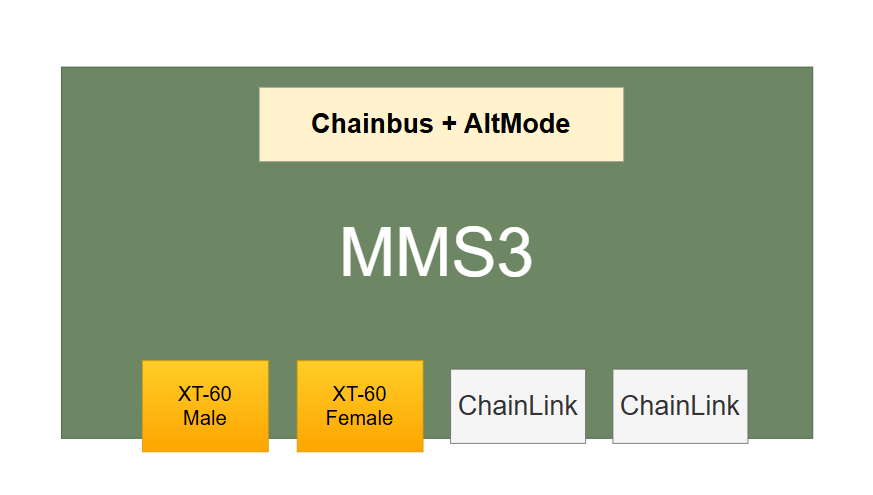
\includegraphics[width=0.5\textwidth]{photos/MMS3_MCU_Top_view.png}
  \caption{Widok kontrolera MMS3 z góry}
  %\label{fig:NoLabel}
\end{figure}


\section{MiniModuCard - Hat} \label{MiniModuCard - Hat}
Hat to ta płytka, która faktycznie coś robi w MiniModuCard. Do niej są podłączone
czujniki, silniki i wszystko inne.

\subsection{Złącza}
\begin{itemize}
  \item 2x ChainBus (jeden na dole, jeden na górze) do podłączenia hatów.
  \item 2x XT60 jeśli potrzebujesz więcej zasilania.
  \item 1x 4-pin złącze do flashowania EEPROMA.
  \item I złącza JST-XH, do których faktycznie podłączasz to, co musisz.
\end{itemize}

\subsection{Modularność}
Na jednym hacie jest tylko jedna rzecz - osobny hat na serwo, osobny na czujniki odległości itd.
Dzięki temu każdy hat jest łatwo zaprojektować i łatwo je przenosić między projektami.

Do jednego MMS3 można podłączyć do 8 hatów. Jeśli potrzebujesz więcej, to musisz dodać nowy kontroler
MiniModuCard ze swoją wieżą hatów.

\subsection{Krawędzie}
Mamy 4 krawędzie, powiedzmy NEWS jak kierunki świata:
\begin{itemize}
  \item N, długa górna - tam jest ChainBus.
  \item E, krótka prawa - tam są diody LED, zworki konfiguracyjne i przyciski.
  \item W, krótka lewa - ta zostaje pusta.
  \item S, długa dolna - tam są złącza XT60 i JST-XH.
\end{itemize}



\subsection{Rysunek hata}

\begin{figure}[H]
  \centering
  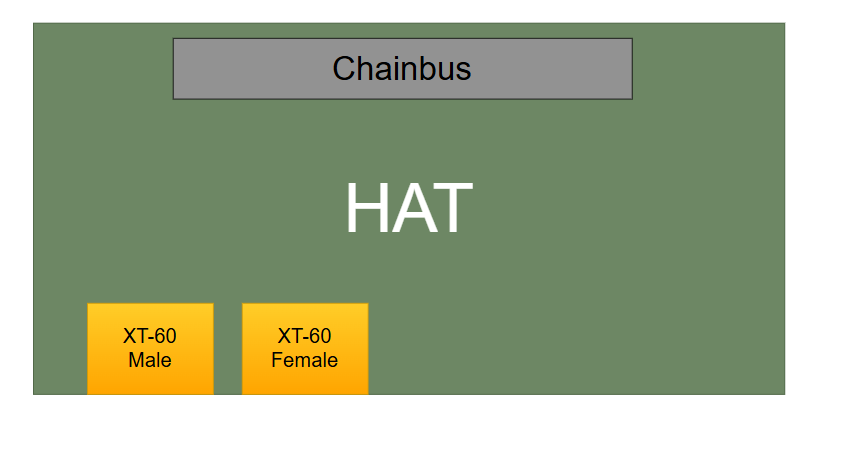
\includegraphics[width=0.5\textwidth]{photos/MMS3_Hat_Top_view.png}
  \caption{Widok hata z góry}
  %\label{fig:NoLabel}
\end{figure}



\section{MiniModuCard - Łączenie hatów}
Na początku masz kontroler MMS. Do niego wpinasz kolejne haty. Kontroler ma złącze albo 3x16, albo 2x16 goldpin żeński THT.
Do niego wpinasz hata. Ten pierwszy hat ma z dołu złącze 2x16 goldpin męski SMD, które wpinasz do MMS3.
I teraz na pierwszym hacie na górze masz złącze 2x16 goldpin żeński SMD, do którego możesz wpiąć kolejnego hata.

\begin{figure}[H]
  \centering
  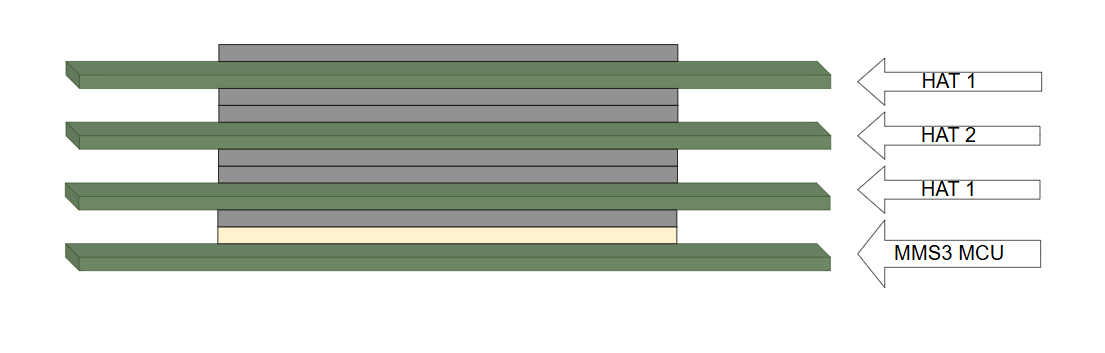
\includegraphics[width=0.5\textwidth]{photos/MMS3_Tower_Side_view.png}
  \caption{3 haty wpięte w Kontroler MMS3}
  %\label{fig:NoLabel}
\end{figure}

\begin{itemize}
  \item To żółte to złącze z kontrolera MMS3.
  \item A czarne to złącza hatów. Dolny jest męski, górny żeński.
\end{itemize}

\section{Wybieranie hatów} \label{sec:wybieranie_logika}
Haty są podpięte przez bus switche, które odpinają i podpinają magistrale. Tak wygląda wybieranie:

\subsection{Jak to działa}
MMS3 MCU ma 8 pinów, ADDR1 do ADDR8. Służą do adresowania hatów. Poprzez wystawianie
na odpowiednie HIGH albo LOW można wybierać haty.

\subsection{Wybieranie}
Bus switche na hatach mają odwróconą logikę. Jak dostają 3V3, to są wyłączone, a jak 0V, to podpinają hata do magistral.
Każdy hat patrzy tylko na swoją linię ADDR1, a resztę przekazują dalej.

\subsection{Przesunięcie}
Z MMS piny ADDR idą prosto na pierwszego hata. Ale z hatów idą już na skos - linia
ADDR3 idzie na ADDR2, ADDR2 na ADDR1 itd. Linia wchodząca na ADDR1 jest używana przez hata
i nieprzekazywana dalej.

\begin{figure}[H]
  \centering
  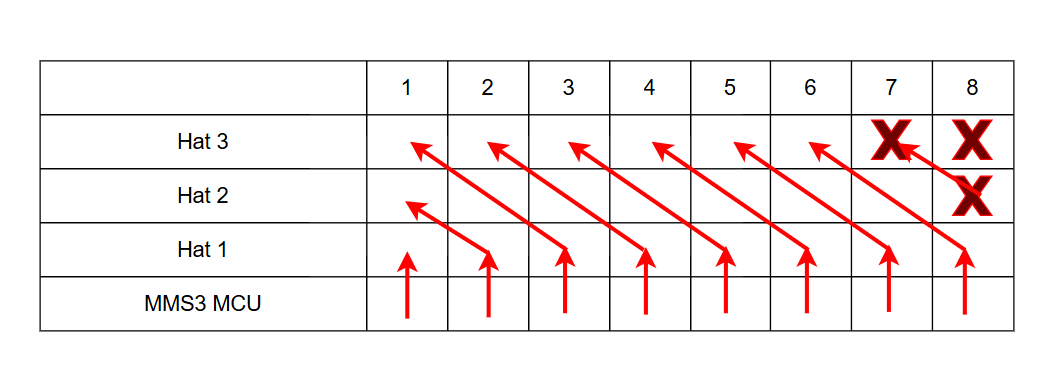
\includegraphics[width=0.5\textwidth]{photos/MMS3_hat_selecting_diagram.png}
  \caption{Tak wyglądają te połączenia hatów i MMS3}
  %\label{fig:NoLabel}
\end{figure}

\subsection{Przykład}

MMS3 chce wybrać 3. hat.
\begin{itemize}
  \item Zaczynamy z punktu wyjścia, wszystkie ADDR są na 3V3 (HIGH), czyli logiczne 0. Żaden hat nie jest wybrany.
  \item MMS3 ustawia ADDR3 na LOW.
  \item Pierwszy hat widzi, że ADDR3 jest LOW, reszta HIGH. Jego ADDR1 jest HIGH, czyli nie reaguje.
  \item Drugi hat widzi, że ADDR2 jest LOW, reszta HIGH. Jego ADDR1 jest HIGH, czyli nie reaguje.
  \item Trzeci hat widzi, że ADDR1 jest LOW, reszta HIGH. Jego ADDR1 jest LOW, czyli się aktywuje.
  \item MMS3 komunikuje się z hatem 3.
  \item MMS3 ustawia ADDR3 na HIGH, hat się wyłącza.
  \item I wracamy do punktu wyjścia, można aktywować kolejny hat.
\end{itemize}

To jest tylko komunikacja, tak to haty pracują w tle (np. czujniki temperatury mogą się kalibrować,
silniki kręcić ze stałą prędkością etc).

\begin{figure}[H]
  \centering
  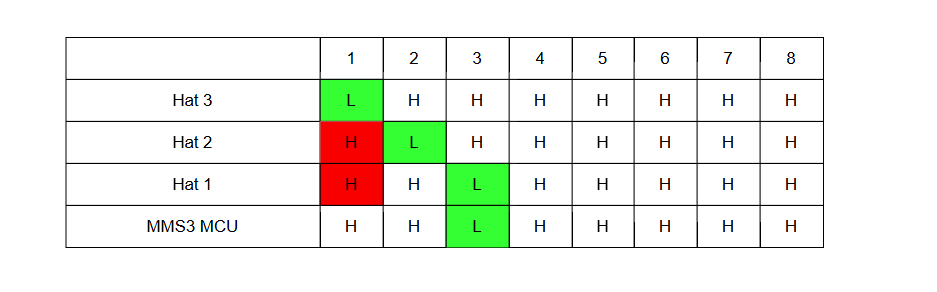
\includegraphics[width=0.5\textwidth]{photos/MMS3_hat_selecting_example.png}
  \caption{To, o czym właśnie napisałem}
  %\label{fig:NoLabel}
\end{figure}


\section{MiniModuCard - Interfejsy i protokoły komunikacyjne}
\subsection{MMS3 a haty}
MMS3 i haty komunikują się po SPI, I2C i UART przez złącze ChainBus.

\subsubsection{I2C}
Normalne I2C, ale każdy hat ma osobną pulę adresów. Adres 1010000 jest zajęty
przez EEPROM (np. M24C64 z A0 A1 A2 zwartymi do masy). EEPROM ma dane identyfikacyjne (nazwa, UUID, hardware revision, software revision)

\subsubsection{SPI}
No, normalne SPI. Jak potrzebujesz mieć więcej slave'ów niż 1, to zabraknie ci Chip Select.
Polecam dać ekspander GPIO po I2C albo zaimplementować expander na CH32V003, bo jest tańszy.

\subsubsection{UART}
UART. Pamiętaj, że podpinasz się do hatów tylko na chwilę, więc nie możesz cały czas nasłuchiwać
RX. Chcesz wysłać coś po TX i dostać odpowiedź.

To, albo dać jakiś MCU (CH32V003) na hat'a który przetłumaczy z UART na SPI albo I2C.

Oh, i ja już się pomyliłem i zamieniłem TX z RX. Tak to ma wyglądać:
\begin{figure}[H]
  \centering
  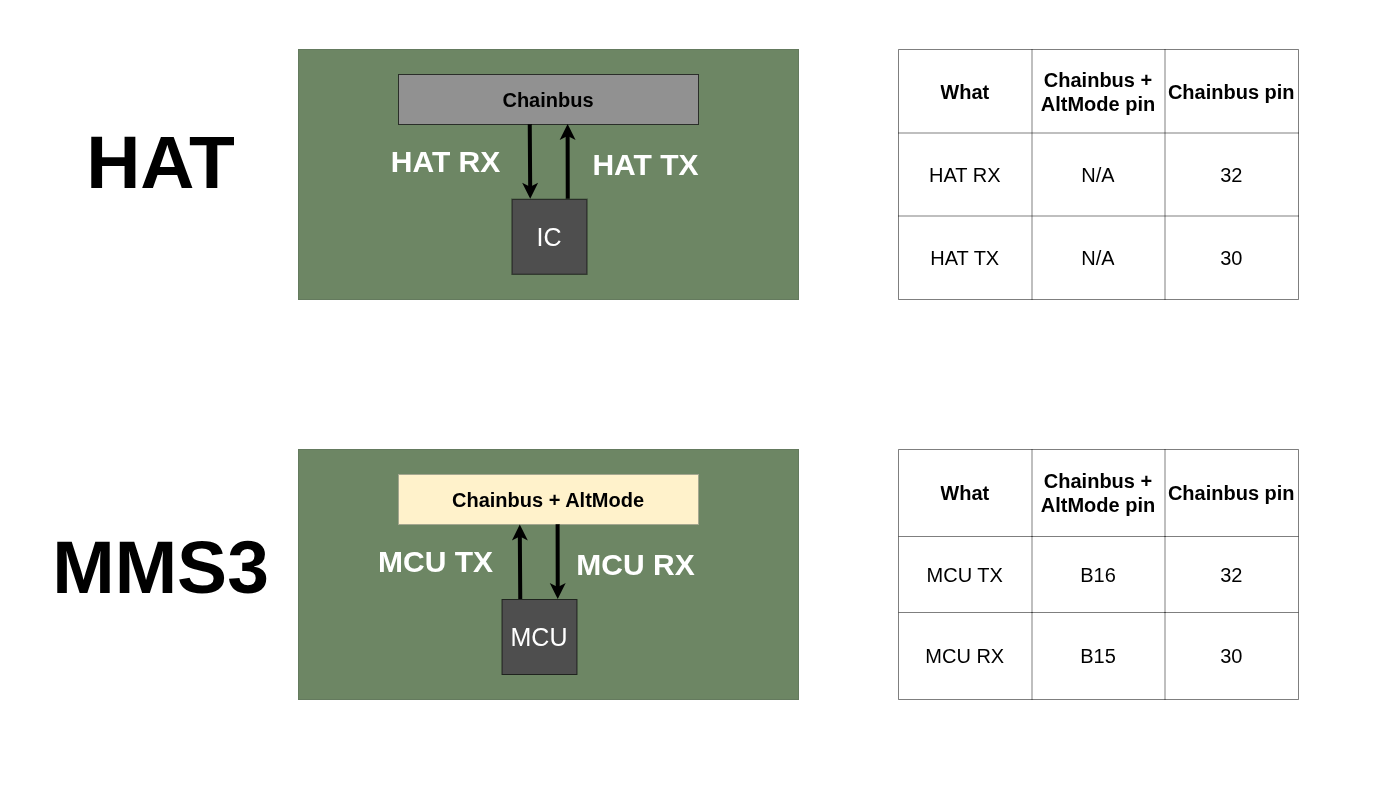
\includegraphics[width=1\textwidth]{photos/MMS3_Uart_Flip_Situation.png}
  \caption{Gdzie jest TX i RX}
  %\label{fig:NoLabel}
\end{figure}



\subsection{MMS3 a główny komputer ModuCard}
MMS3 komunikuje się z komputerem pokładowym ModuCarda po ChainLink.
\subsubsection{CAN}
Są 2 linie CAN w ChainLink. Jakoś to gada. Problem programisty. Jak jesteś programistą, to masz problem.
% /#\#/\/#\ Trzeba coś tu dopisać
\subsubsection{USB}
Jest 1 linia USB. Można się nią podłączyć do MMS3 i go programować po niej.

\subsection{Programowanie i debugowanie}
Więc hata da się debugować po USB-C.
\subsubsection{USB hub}
MMS3 ma wbudowanego huba USB i programator. Więc każdego MMS3
możesz debugować jednym kablem, bo masz USB hub -> Mikrokontroler (więc możesz użyć np. USB serial)
i masz USB hub -> programator -> mikrokontroler (więc możesz wgrywać program przez to USB).
\subsubsection{USB-C a ChainLink}
Więc to jest opcja debugowania i flashowania lokalnego. Możesz też robić to samo z poziomu głównego komputera ModuCard
przez ChainLink, bo do niego idzie USB przez ChainLink. MMS3 ma przełączniki USB, które automatycznie
przełączają się między USB-C a ChainLinkiem. Normalnie jest do ChainLinka, ale jak się podłączysz kablem,
to priorytet ma kabel.

\subsubsection{Sznurek/gałąź MMS3}
Każdy MMS3 ma 2 złącza ChainLink, więc możesz je daisy-chainować (łączyć pierwszy z kolejnym i tak dalej).
Dzięki temu musisz wyprowadzić tylko jedno złącze ChainLink z ModuCarda i do tego możesz podłączyć ile chcesz MMS3.

% /#\#/\/#\ Ile konkretnie
Adnotacja: Chyba huby USB mają limit, ile ich można dać za sobą, albo signal integrity USB się spierdzieli.
Czyli jest jakiś limit, jak będę wiedział jaki, to napiszę.

\section{MiniModuCard - AltMode i stopnie integracji} \label{AltMode}

\subsection{O co chodzi z rzędem AltMode}
MMS3 ma 3 rzędy pinów, a hat tylko 2. Wątek jest taki: mikrokontrolery zwykle mają więcej
pinów niż potrzeba na sam ChainBus, więc te luźne wystawiliśmy na 3. rząd. Oto dlaczego:

Normalnie MMS3 używamy z ChainBusem + hatami, więc mamy wszystkie zalety modularności etc.
Fajnie wszystko idzie, jak prototypujesz albo rozwijasz projekt. Ale gdybyś chciał bardziej zintegrować,
pomniejszyć projekt, to możesz zrobić hata AltMode.

Pinout rzędu AltMode jest inny dla każdego MMS3.

\subsection{A z hatem AltMode?}
Jak już masz przetestowane układy i kod, to możesz swoje 8 hatów połączyć w jednego dużego. Teraz możesz
użyć pinów AltMode i adresowania jako zwykłe GPIO i nowe magistrale komunikacyjne. Wtedy
na jednego MMS3 wpinasz jedną dużą płytkę, która robi to samo co 8 hatów.

Już raczej jej nie będziesz przenosił między projektami, ale to jest tylko do finalizacji projektów.
I dalej, możesz na tę samą płytkę dać samego MMS3 i mieć cały projekt na 1 PCB.

Zaleta od zaczęcia tak zaraz zamiast skipnięcia od razu do 1 PCB jest taka, że możesz wszystko stopniowo testować, łatwo modyfikować i
tanio prototypować.

W kole nie używamy ani AltMode, ani stopniów integracji projektu 2 i 3. (At least for now)

\subsubsection{Stopnie integracji}
\begin{itemize}
  \item Stopień 1 - MMS3 + 8 hatów ChainBus.
  \item Stopień 2 - MMS3 + 1 hat AltMode.
  \item Stopień 3 - Wszystko na tym samym PCB.
\end{itemize}

To jest pierwszy wątek, w praniu jeszcze wyszedł drugi wątek: co jak programista bardzo krzyczy że potrzebuje interruptów a w chainbus'ie nie ma interruptów?

Oto kolejność postępowania

1. Powiedz mu że ma skill issue i że to da rade zaprogramować bez nich na polling

2. Możesz dać jakiś MCU na hat'a który obsłuży twój układ z interruptami i przekaże te dane do głównego proca MMS3

3. Zastanów się czy nie lepiej zrobić to na Karcie dużego ModuCard'a

4. Możesz zrobić hat'a altmode. Czyli nie używasz chainbus'a i wykorzystujesz piny MMS3 jako GPIO. Robisz jedną płytke która wpina się do wszystkich trzech rzędów MMS'a. Wtedy masz jedną płytke na jednego MMS3, bez chainbus'a ale masz interrupty and all that jazz. 

Spoko w czwartej opcji jest że możesz podłączyć kilka MMS3 ze sobą i na jednym mieć altmode'a bo go bardzo potrzebujesz a na reszcie chainbus. One gadają po CAN więc jest git.

\section{MiniModuCard - Przykładowe MMS-y i haty}
\subsection{MMS3}
\begin{figure}[!h]
  \centering
  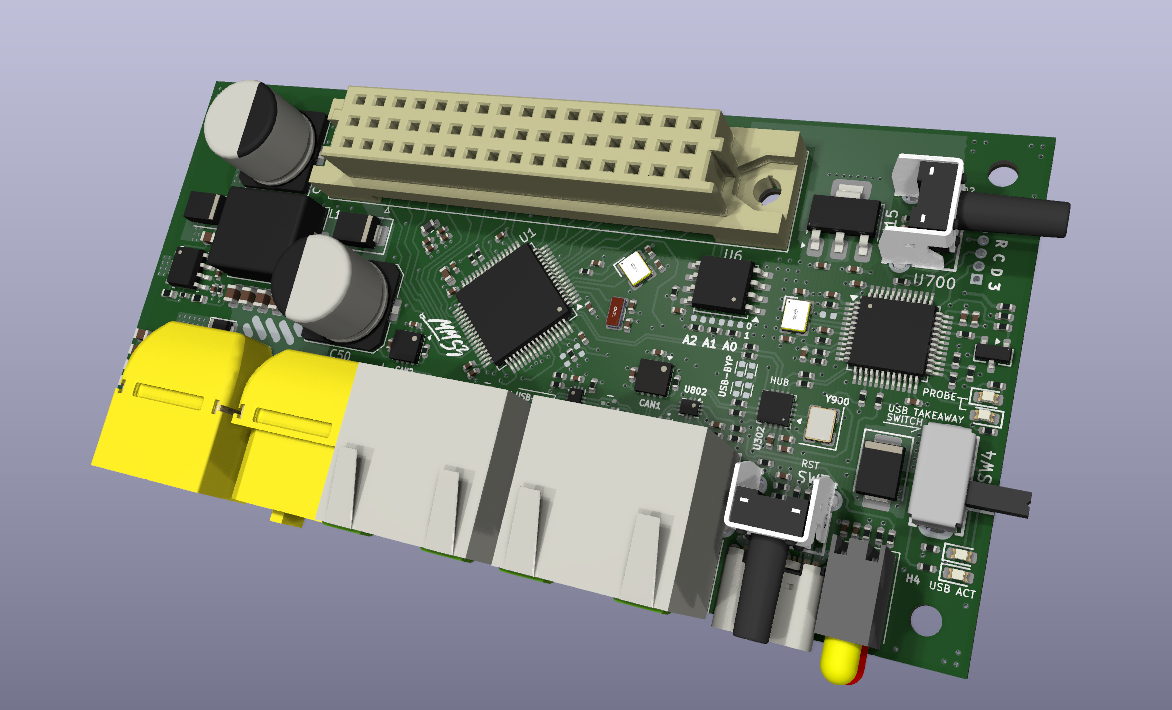
\includegraphics[width=0.5\textwidth]{photos/MMS3.png}
  \caption{MMS3 STM32F405}
  %\label{fig:NoLabel}
\end{figure}


\subsection{Haty}


\begin{figure}[!h]
  \centering
  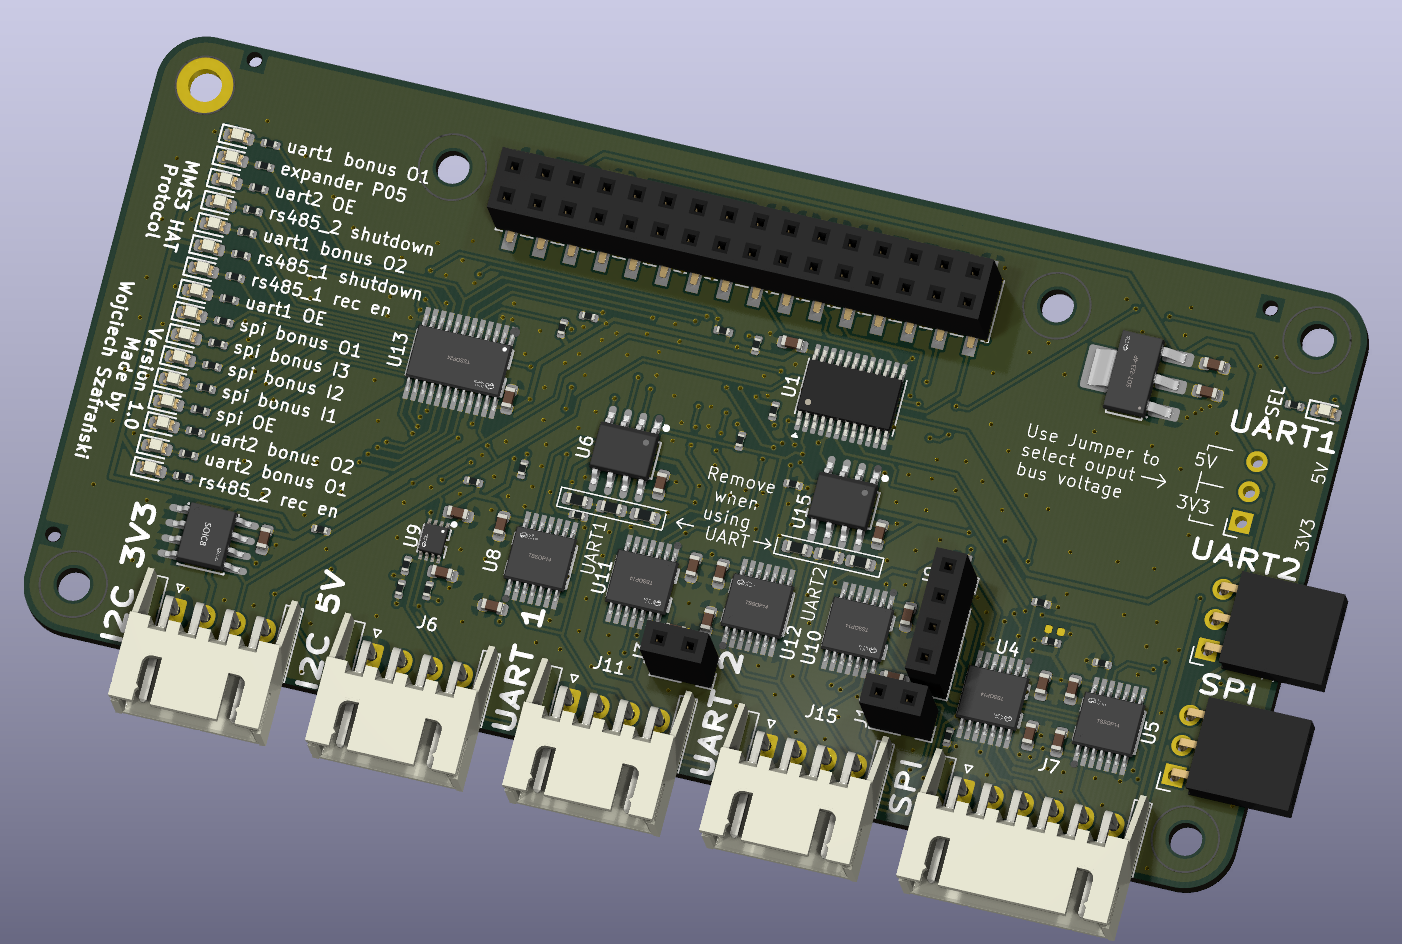
\includegraphics[width=0.5\textwidth]{photos/MMS_hat_protocol.png}
  \caption{Hat protocol}
  %\label{fig:NoLabel}
\end{figure}

\begin{figure}[!h]
  \centering
  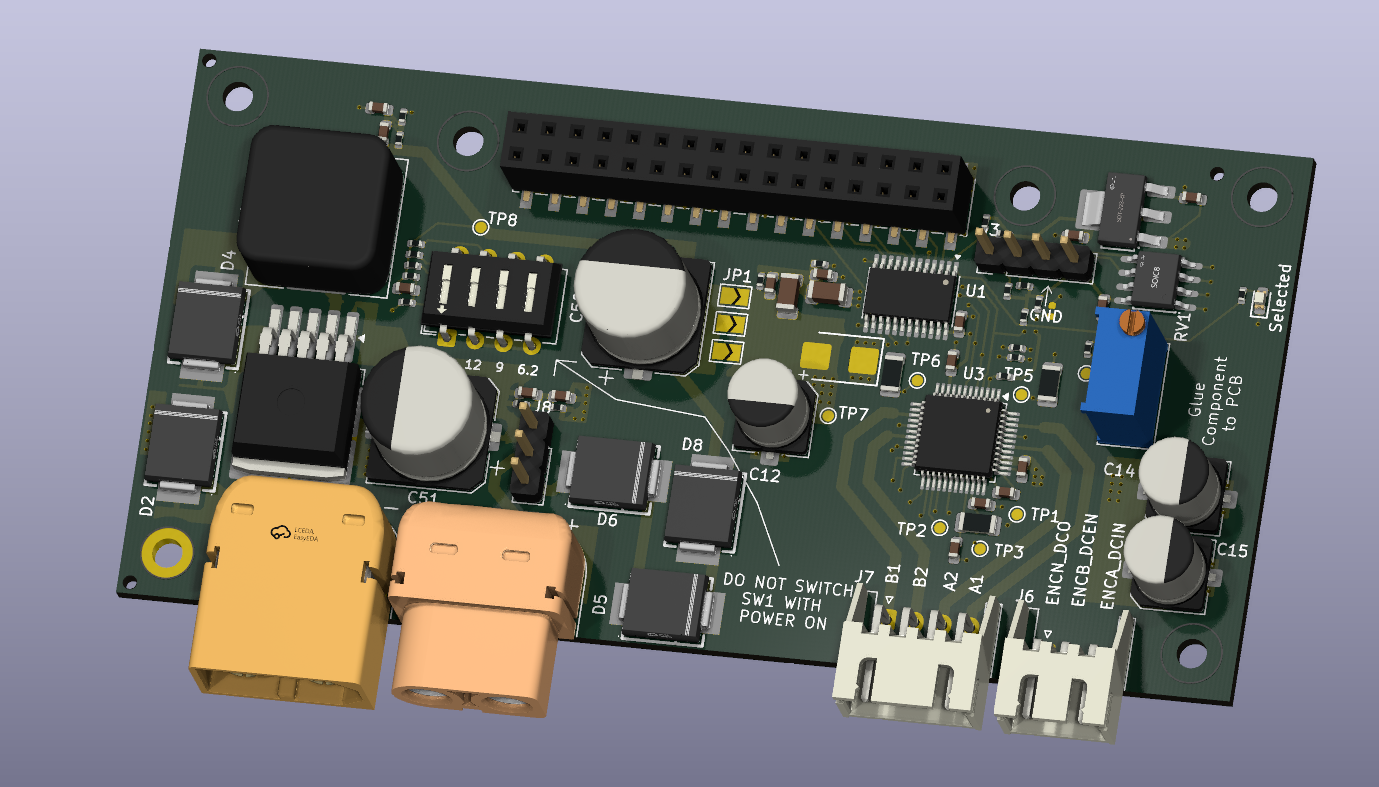
\includegraphics[width=0.5\textwidth]{photos/MMS_hat_stepper.png}
  \caption{Hat stepper}
  %\label{fig:NoLabel}
\end{figure}

\begin{figure}[!h]
  \centering
  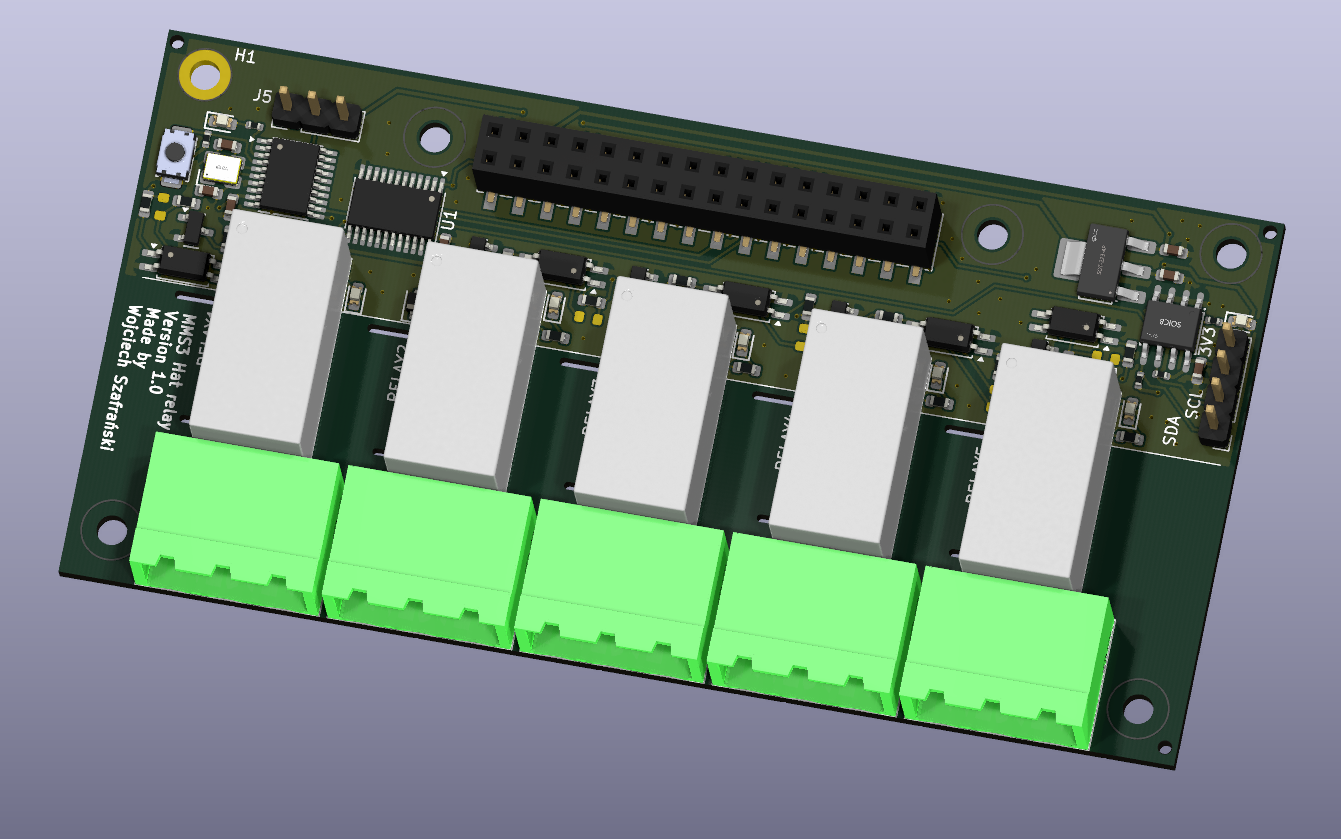
\includegraphics[width=0.5\textwidth]{photos/MMS_hat_relay.png}
  \caption{Hat relay}
  %\label{fig:NoLabel}
\end{figure}

\begin{figure}[!h]
  \centering
  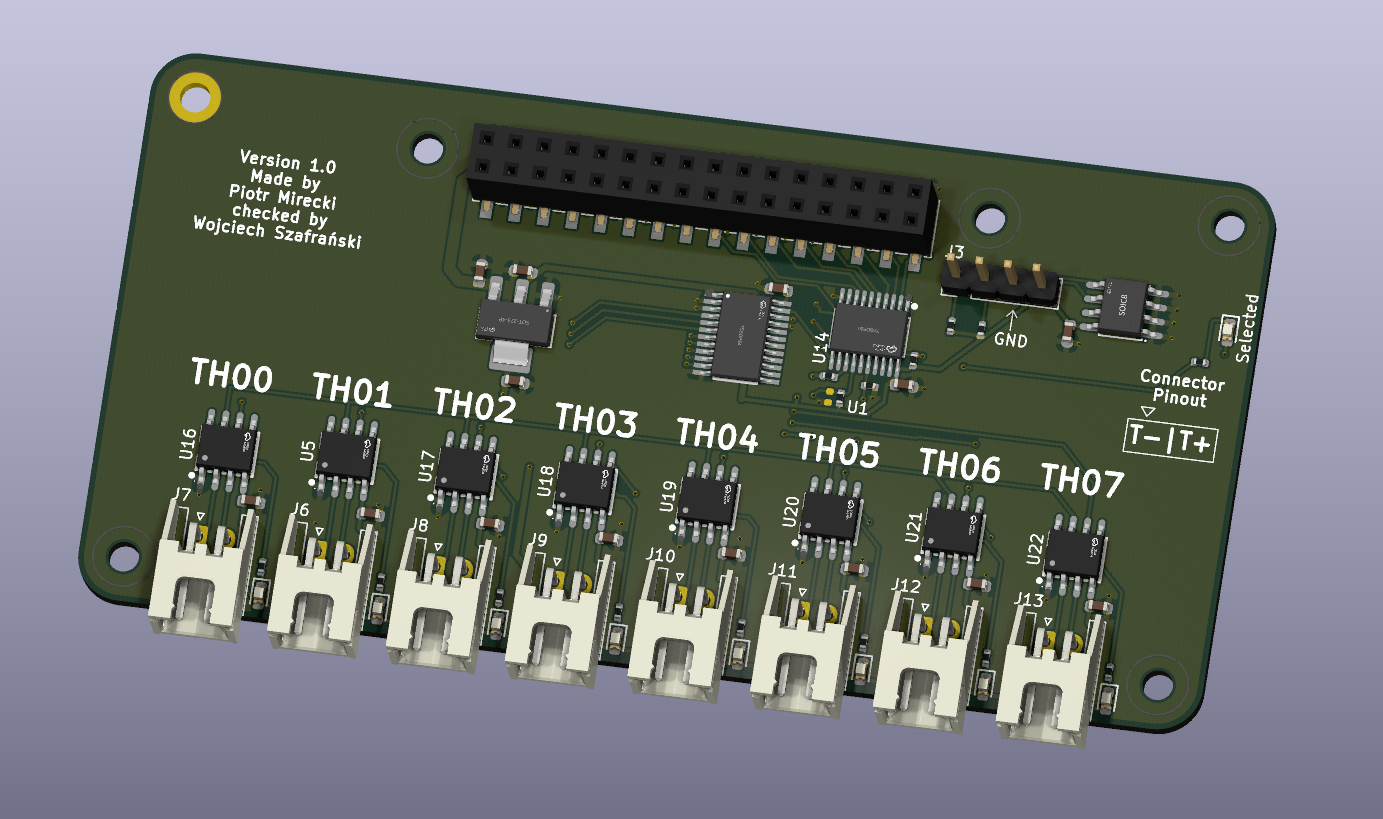
\includegraphics[width=0.5\textwidth]{photos/MMS_hat_thermocouple.png}
  \caption{Hat thermocouple}
  %\label{fig:NoLabel}
\end{figure}

\newpage

% /#\#/\/#\ Opis TBD
\section{MiniModuCard - Budżet mocy}


Normalnie MMS3 zasilasz ze złącza XT60 i to idzie na BRD VIN. MMS3 ma obowiązek zrobić z tego
przetworkę BUCK DC-DC na 5V co najmniej 1A. 12V Standby nie używajcie. I ChainBus za dużo
nie puści prądu BRD VIN przez siebie, więc jak hat pobiera więcej prądu niż jakieś 185mA z niego,
to dajcie XT60 na swojego hata. Ona może puścić max 60A.

Więc jak mamy np. 1A 5V, to jak dasz 8 hatów, to każdy może pociągnąć 125mA. Ale jak dasz tylko 2 haty,
to już każdy może pociągnąć 500mA. A niektóre haty mogą ciągnąć mniej, jak mają np. same czujniki.

Na dole masz mniej więcej limity, staraj się ich nie przekraczać, a jak przekraczać to ostrożnie:
\begin{table}[h]
  \centering
  \renewcommand{\arraystretch}{1.5}
  \begin{tabular}{|l|c|c|c|}
    \hline
    \textbf{Nazwa} & \textbf{Napięcie} & \textbf{Sumaryczny prąd} & \textbf{prąd na jeden hat} \\ \hline
    5V             & 5.0 V             & 1.0 A                    & 125 mA                     \\ \hline
    12V stby       & 12.0 V            & 0.5 A                    & 65 mA                      \\ \hline
    BRD\_VIN       & 12.0 V -- 48.0 V  & 1.5 A                    & 185 mA                     \\ \hline
  \end{tabular}
\end{table}


Komponenty podłączone do linii \texttt{BRD\_VIN} muszą być przystosowane do pracy z napięciem od 12V do \textbf{48 V}.


\section{MiniModuCard - Wymagania dla hata}
Tbh większość z tego jest już na templatce:

\begin{itemize}
  \item Wymiary 100x50mm.
  \item Ma 6 otworów montażowych M2.5.
  \item Nie daje komponentów na keepout zone'ach (zob. sekcja mechaniczna).
  \item I komponenty tylko z przodu, nie wyższe niż XXXmm. % /#\#/\/#\
  \item Złącza XT60 są na długiej krawędzi.
  \item Złącza wyjściowe są na długiej krawędzi.
  \item Złącza wyjściowe mają raster 2.54mm i używamy JST-XH.
  \item Zworki konfiguracyjne są na prawej krótkiej krawędzi.
  \item Przyciski, LED-y też na prawej.
  \item lol lewa jest wolna.
  \item Złącze ChainBus w dobrym miejscu, z góry female i z dołu male.
  \item ChainBus przesuwa piny ADDR, reszty nie.
  \item Obsługuje napięcie na BRD VIN do 48V.
  \item Nie pobiera więcej prądu niż z budżetu mocy (kinda whatever).
  \item Podłącza ChainBus tylko do SPI, I2C, UART i nie odwala nic dziwnego z nimi.
  \item Nic dziwnego, między innymi sam nie zaczyna komunikacji, tylko grzecznie czeka na MMS3 aż zacznie gadać.
  \item Podłącza magistralę tylko kiedy ADDR1 = LOW.
  \item Ma EEPROM do identyfikacji po I2C o dobrym adresie i zgodnej komunikacji.
  \item Ma złącze I2C (3V3, GND, SCL, SDA) na prawej krawędzi, żeby łatwo flashować EEPROM.
  \item Ma diodę, która się świeci, jak hat jest wybrany.
  \item Ma pull-upy/downy na komunikacji (i ADDR1), żeby nie była floating jak hat jest odpięty.
  \item Jest w licencji TO-DO. % /#\#/\/#\
  \item Ma zdjęcie, BOM na GitHubie.
  \item Ma dokumentację na GitHubie.
  \item Ma soft na GitHubie.
  \item Ma tagi hashtag XXX na dole dokumentacji, żeby dało radę go wyszukać. % /#\#/\/#\ zrób
  \item Wszystkie złączki mają opisany pinout na silkscreenie.
  \item Nazwa, autor i rewizja hata jest opisana na silkscreenie.
  \item Duuużo diod, żeby się ładnie świeciło.
  \item Same złączki też opisane do czego są dużymi literami, żeby było ładnie.
\end{itemize}
\section{MiniModuCard - Wymagania dla MMS-a}
\begin{itemize}
  \item Jakiś proc na nim.
  \item Złącza XT-60.
  \item Przetworka VBUS -> 5V 1A.
  \item Przełączanie ADDR.
  \item Obsługa protokołów na ChainBus.
  \item Wymiary, złącza i otwory w dobrych miejscach.
  \item Przełączanie USB między złączką C a ChainLinkiem.
  \item USB hub na programator i USB z MCU.
  \item Obsługa ChainLink.
  \item 2x CAN.
\end{itemize}
\section{MiniModuCard - Projektowanie hatów} \label{MiniModuCard - Projektowanie hatów}
\subsection{Co musisz zrobić}

Jeśli tu jesteś, to znaczy, że ktoś cię poprosił o zrobienie Hat'a do MiniModuCard'a. W tej książce jest cała dokumentacja systemu, ale postaram się streścić najważniejsze rzeczy, które musisz wiedzieć tutaj.

Zakładam, że dostałeś zadanie w stylu "zrób hat'a, który odbiera GPS", "który steruje silnikiem BLDC" albo "zrób hata z układem scalonym DRV17182". Jeśli się zgadza, to możesz czytać dalej.

\subsection{Co musisz wiedzieć}
Powinieneś przeczytać Primer (\ref{Primer}), zasadę działania MiniModuCard'a (\ref{MiniModuCard - zasada działania}) oraz sekcję o Hat'ach (\ref{MiniModuCard - Hat}).

Pozwolę sobie założyć, że tego nie zrobiłeś, i na szybko jeszcze raz to opiszę.

\subsubsection{Co to hat}

Mamy system, w którym jest płytka z mikroprocesorem (np. STM32F405) i chcemy, żeby coś robiła. Żeby to było modularne, oddzieliliśmy procesor i układy wyjściowe na osobne płytki. Te osobne płytki z układami wyjściowymi to są "Hat'y" i ty takiego masz robić.

Mówiąc układ wyjściowy, mam na myśli np. właśnie sterownik silnika albo moduł GPS. Cokolwiek,
co coś odczytuje albo steruje poza płytką.

Inaczej mówiąc, hat to tak jakby shield na Arduino.

\subsubsection{Jak to działa}

Procesor ma swoje piny (W arduino są wyprowadzone na te czarne złacza do których podłaczasz moduły). One zmieniają swoje napięcia i sterują rzeczami. Są wyprowadzone na złącze ChainBus i przez nie do każdego hat'a.

Konkretnie, do hatów jest doprowadzone I2C, SPI i UART. To są takie mega często stosowane protokoły komunikacyjne. Ich będziesz używać do sterowania układami scalonymi (IC) na hat'ie.

Twoje zadanie to znaleźć układ, który robi to, co chcesz (np. sterownik termopary) i to taki, żeby komunikował się po I2C, SPI albo UART, a nie jakimś dziwnym własnym protokołem. Jak już znajdziesz, to zapytaj się osoby, od której dostałeś zadanie zrobienia płytki, czy będzie pasował.

Jak masz ten układ wybrany, to musisz narysować w programie "KiCad", do czego jest podłączony. To jest schematic. Potem przenosisz go na fizyczną płytkę w tym samym programie. Wtedy masz PCB.

(Jeszcze jest system automatycznego wybierania Hat'ów przez piny ADDR, ale nie musisz się
o nim martwić, bo już jest na templatce).

\subsection{Templatka}
Żeby było łatwiej projektować, to zrobiłem projekt z podstawowymi elementami hat'a na GitHubie,
który możesz z'fork'ować i na nim projektować.

Link -> \url{https://github.com/KoNaR-Hefajstos/MMS3_hat_templates}

Tak wygląda otworzony w programie KiCad (musisz wejść w widok schematu/płytki)

\begin{figure}[H]
  \centering
  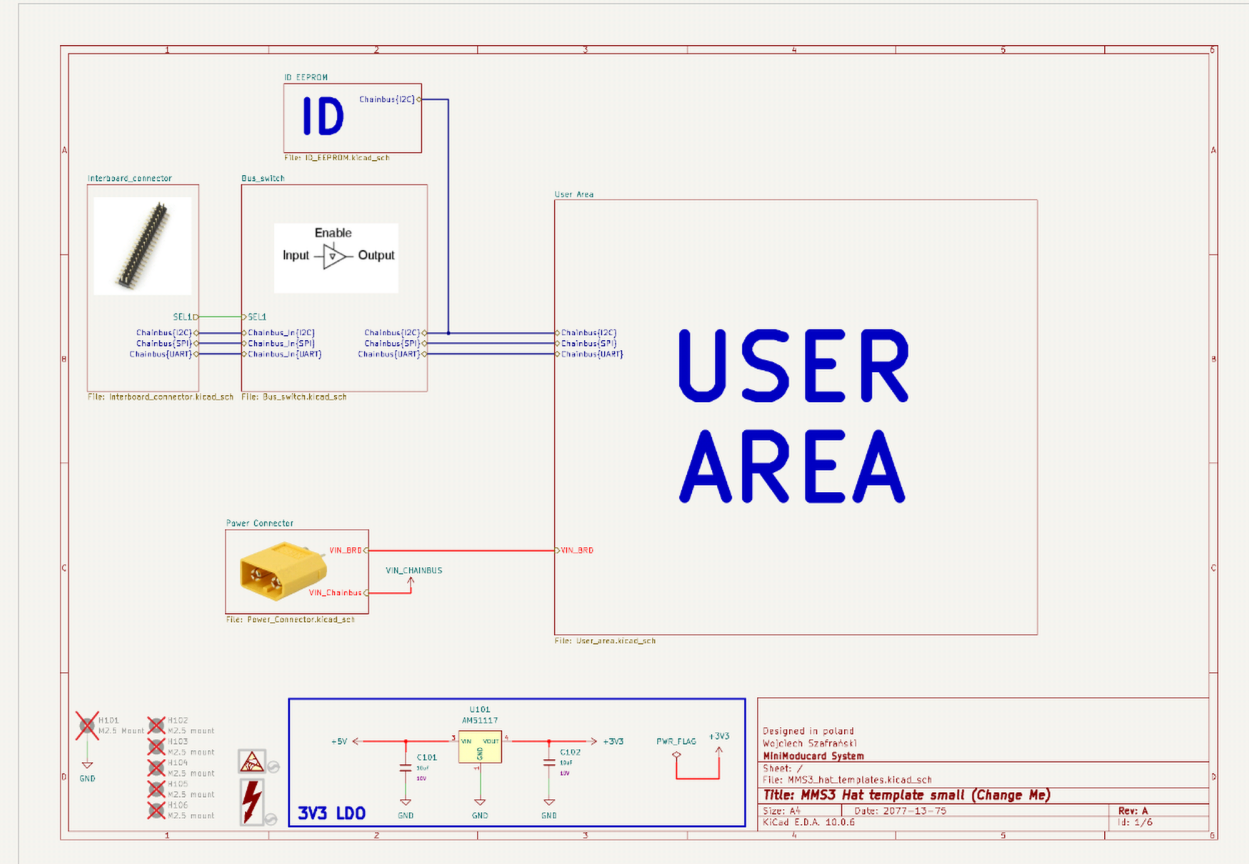
\includegraphics[width=0.8\textwidth]{photos/MMS3_hat_template_schematic.png}
  \caption{Widok schematic templatki}
  %\label{fig:NoLabel}
\end{figure}

\begin{figure}[H]
  \centering
  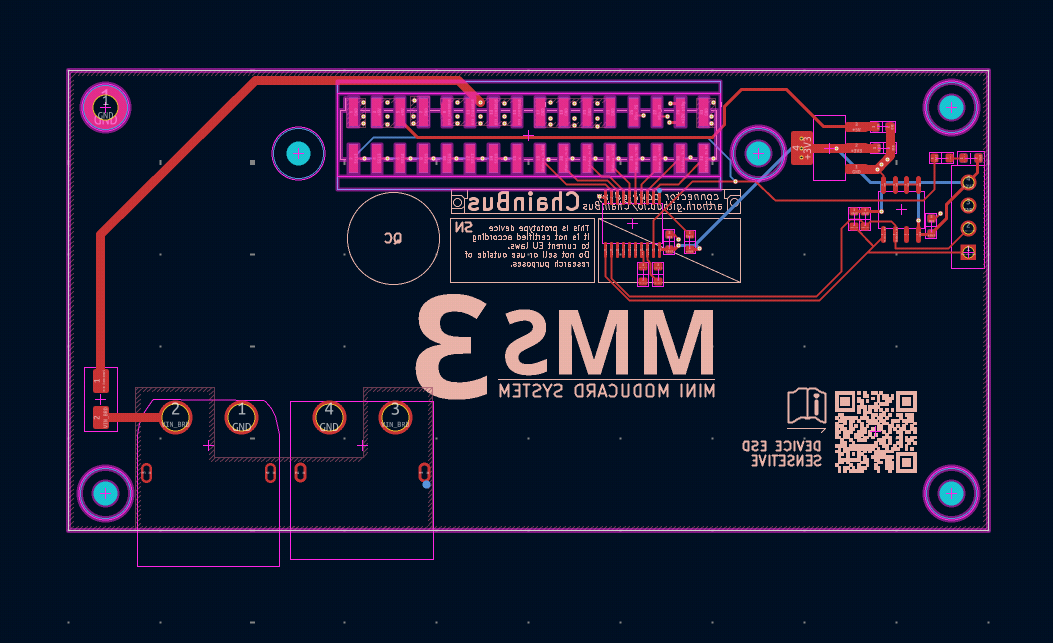
\includegraphics[width=0.8\textwidth]{photos/MMS3_hat_template_pcb.png}
  \caption{Widok płytki PCB templatki}
  %\label{fig:NoLabel}
\end{figure}

(Zdjęcia mogą być stare, są z 4.09.26)

\subsubsection{Noteworthy rzeczy o templatce}
\begin{itemize}
  \item Masz już zrobione złącze ChainBus, adresowanie i resztę
  \item Co potrzebujesz dodać na schematic'u, dodaj w środku "User area". Reszty nie dotykaj ale polecam sobie obejrzeć jak to działa.
  \item Okay, jedyną rzeczą którą możesz ruszyć jest "Power Connector". To jest złącze XT60 i możesz go usunąć ze schematic'a i PCB jeśli go nie potrzebujesz (ono służy do podlączenia więcej zasilania jak musisz mieć więcej prądu na VIN niż chainbus ci da)
  \item Nie zmieniaj rozmiaru płytki PCB i nie ruszaj rozstawu śrub montażowych oraz złącz ChainBus.
  \item Schematic jest podzielony na hierarchical sheet'y (np. Bus switch. Te prostokąty, możesz na nie dwa razy kliknąć, żeby zobaczyć do środka). Proszę też ich używaj <3
  \item O, i co do hierarchical sheet'ów (schematów hierarchicznych), to możesz zobaczyć, czy na innym hat'ie nie ma jakiegoś, który ci się przyda. Powinny być opisane w README
\end{itemize}

Basically musisz dodać swój układ i połączyć z jedną/dwoma/trzema protokołami komunikacyjnymi w środku User Area. I nie usuwać/przesuwać ważnych rzeczy.

Parę jeszcze rzeczy jest napisane w README template'a.

\subsection{Setup programów}
\begin{itemize}
  \item Musisz zainstalować KiCad'a \url{https://www.kicad.org}
  \item I te pluginy do niego:
  \item Do generowania pliku BOM (Bill of materials) \url{https://github.com/openscopeproject/InteractiveHtmlBom}
  \item Do generowania plików produkcyjnych (tzw. gerber) \url{https://github.com/Bouni/kicad-jlcpcb-tools}
  \item Do pobierania footprint'ów komponentów z LCSC \url{github.com/hulryung/kicad-lcsc-manager} 
  \item Biblioteka podstawowych komponentów z JLCPCB assembly: \url{https://github.com/CDFER/JLCPCB-Kicad-Library}
\end{itemize}

\subsection{Jak robić schematic/PCB}
Pełne tłumaczenie od zera jest out of scope tego dokumentu (wierzę, że znajdziesz jakiś fajny poradnik na YT), ale

\subsection{Pobieranie symboli i footprint'ów - pasywki}
(symbol - element na schematic'u. Jakie ma połączenia. Footprint - element na PCB, jaki ma fizyczny kształt)

Zwykle zamawiamy PCB częściowo zlutowane (basic assembly) z firmy JLCPCB. Trzeba używać komponentów od nich, żeby nie trzeba było ich później ręcznie wybierać przy zamawianiu. Dodatkowym bonusem jest to, że ładnie widać je na modelu 3D.

Elementy pasywne (pasywki - rezystory, kondensatory, LED-y etc) są już pobrane razem z pluginami. Musisz tylko dobre wybrać.
Dobre, to znaczy z kategorii PCM\_JLCPCB.

\begin{figure}[H]
  \centering
  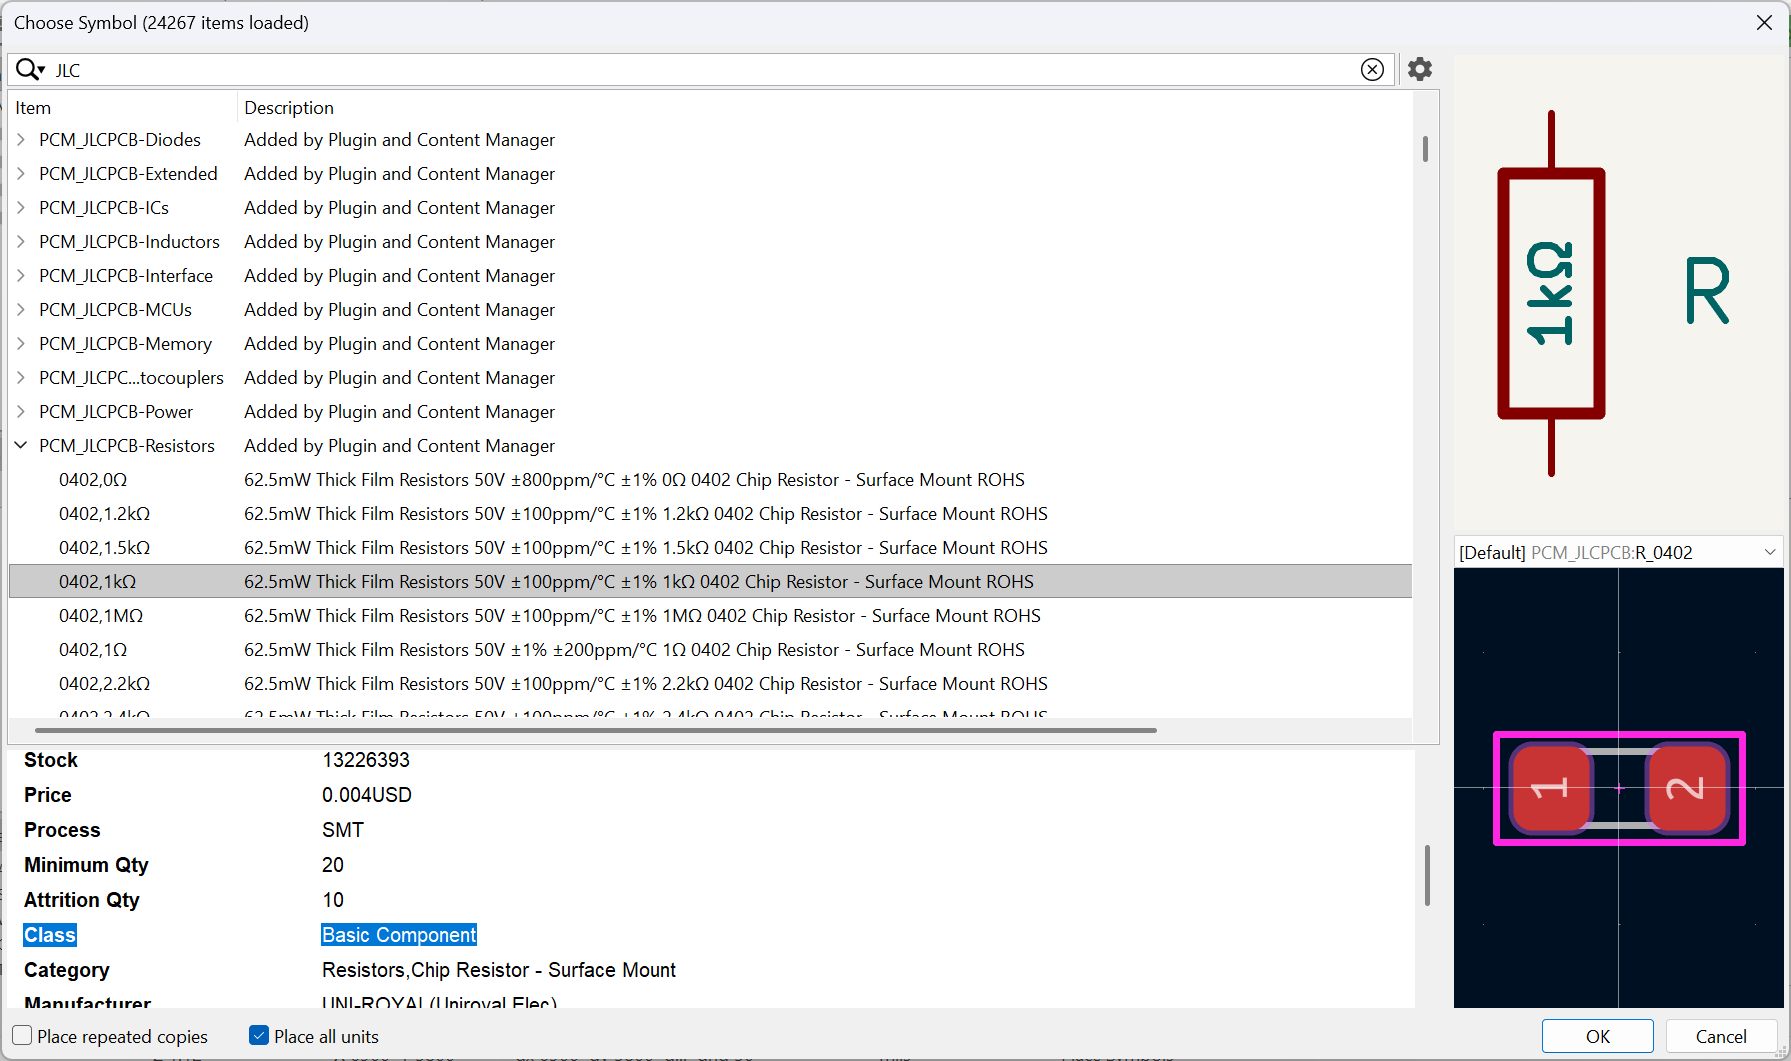
\includegraphics[width=0.8\textwidth]{./photos/KiCad_adding_JLCPCB_components.png}
  \caption{Widok z dodawania komponentów KiCad}
  %\label{fig:NoLabel}
\end{figure}

Staraj się wybierać, jak możesz, komponenty "Basic Component". Za każdy inny komponent trzeba zapłacić dodatkowo 1.5\$ za załadowanie do maszyny pick and place. Zazwyczaj basic będą tylko podstawowe rezystory, kondensatory, diody (w tym LED), oscylatory i parę innych. Pełną listę możesz znaleźć, wchodząc na stronę \url{https://jlcpcb.com/parts} i odfiltrować tylko te basic. 

Najprawdopodobniej płytka będziej zamówiona tylko z basic  więc im więcej takich komponentów użyjesz tym mniej zabawy potem z kupowaniem i lutowaniem reszty części.

\subsection{Pobieranie symboli i footprint'ów - IC}
Jeśli nie ma twojego komponentu automatycznie pobranego do KiCad'a (czyli większość nie-basic), musisz go ręcznie pobrać. Używamy
do tego plugina kicad-lcsc-manager.

A więc, procedura, której ja używam, wygląda tak:
\begin{itemize}
  \item Wejdź na widok płytki PCB
  \item Na górze na pasku wybierz plugin
  \item Znajdź swój komponent
  \item Pobierz
  \item Gotowe!
\end{itemize}

Wcześniej była inna procedura, ale ta jest lepsza i szybsza. whatever

Oh, i nawet jak nie kupujesz komponentów od JLC/LCSC to I tak pobierz od nich symbol i footprint. Tak jest szybciej i lepiej bo nie pomylisz się przy robieniu/wybieraniu footprint'a.



\subsection{Parę moich komentarzy}
\begin{itemize}
  \item Jak możesz, to daj diody LED do czego się da, żeby widać było, że coś się dzieje, jak płytka działa (zob. hat protocol)
  \item Jak skończysz robić PCB, to opisz wszystkie złącza, diody i co się da na silkscreenie (zob. hat HC-SR04-HX711)
  \item Pamiętaj podpisać, jaki to hat, która wersja i kto ją zrobił na płytce na silkscreenie
  \item W KiCadzie jest widok 3D, jak otworzysz PCB. Zobacz go sobie
  \item 1 / 1.5mm wielkości tekstu silkscreen to minimum, żeby było fajnie widać
  \item (ale mniej też widać, tylko że nie fajnie)
  \item Używaj pasywek wielkości 0603
  \item Jeśli układ, który wybrałeś, ma jakieś piny interrupt, to je ignorujesz,
        zostaw je floating (do niczego niepodpięte). Jeśli ma jakieś piny konfiguracyjne, to daj je na zworki goldpin na boku płytki (jeśli trzeba je często przełączać - goldpin kątowy jest spoko) albo przez zworkę lutowalną/rezystor na samej płytce (jeśli mniej często trzeba je przełączać). Tutaj musisz trochę pomyśleć, jak to musisz zrobić, żeby było dobrze. Zapytaj się kogoś, jak nie wiesz
  \item Jako że nie ma wyprowadzonych zwykłych pinów GPIO do hat'a, tylko same protokoły komunikacyjne, to może ci ich brakować. Jeśli będziesz ich potrzebował, to daj expander GPIO po I2C
  \item Robienie schematic'a (co do czego jest podłączone) nie jest trudne. Basically musisz wziąć jakiś "Typical design" z noty katalogowej układu (ang. datasheet) albo płytkę, którą już ktoś zrobił
  \item Jak robisz fork'a, to chcesz, żeby właścicielem repo była organizacja Konar'u (np. Hefajstos), a nie ty, bo jak jest na ciebie, to nie mam dostępu, żeby poprawić płytkę, jak ją sprawdzam
  \item Złącza wyjściowe (to, po co robisz płytkę) daj jako kątowe JST-XH 2.5mm/2.54mm (któreś z tych dwóch)
  \item Złącza konfiguracyjne (jeśli jakieś masz) daj na prawej krawędzi hat'a. Resztę rzeczy na dolną. Lewą zostaw pustą
  \item Jeśli szukasz układu scalonego i są tylko z własnym
        protokołem albo reszta jest droga, to możesz dać po drodze innego proca, np. CH32V003, który to przetłumaczy na I2C/SPI. Napisz do mnie albo innego ogarniętego elektronika, żeby ci to wytłumaczył
  \item Komponenty zamawiamy zwykle albo z TME, Mouser, może Digikey. TME jest preferowane, ale jest drogo i mało komponentów
  \item Jak nie ma rezystora, którego potrzebujesz, to możesz połączyć 2/3 ze sobą. KiCad ma wbudowany do tego kalkulator, szturchnij mnie to ci powiem co i jak (;

\end{itemize}

\subsection{Dodatkowe źródła do obczajenia}

\subsubsection{Spoko miejsca do znalezienia układu/dokumentacji/layoutu}
\begin{itemize}
  \item Moduły do Arduino
  \item \url{https://www.mikroe.com}
  \item DevBoard'y producenta
  \item Noty katalogowe
\end{itemize}

\subsubsection{Spoko filmy/źródła o projektowaniu schematic'ów/PCB}
\begin{itemize}
  \item \url{https://www.youtube.com/@PhilsLab} <- Absolutny GOAT
  \item \url{https://blog.poly.nomial.co.uk/2025-08-10-creating-high-quality-electronics-schematics.html}
  \item GreatScott na yt -> tłumaczy od podstaw w prosty sposób
  \item \url{https://www.youtube.com/playlist?list=PLEBQazB0HUyQ5YJSdCBb79orXaR3Uk5vm} - Poradnik Digikey do KiCad'a. Nie jest idealny, ale spoko jak nigdy go nie otwierałeś jeszcze.
\end{itemize}

\subsubsection{Na zakończenie}
To tyle z tłumaczenia. Jeśli jest coś, czego nie rozumiesz, myślisz, że można lepiej wytłumaczyć albo brakuje zdjęć, to proszę, \textbf{proszę}
napisz mi co. Imo bardzo ważne jest, żeby ta część dokumentacji była zrozumiała, bo początkujący będą ją próbowali zrozumieć.

\section{MiniModuCard - Pinout złączy}
\subsection{ChainBus + AltMode}
Jest na MMS3.

\begin{figure}[H]
  \centering
  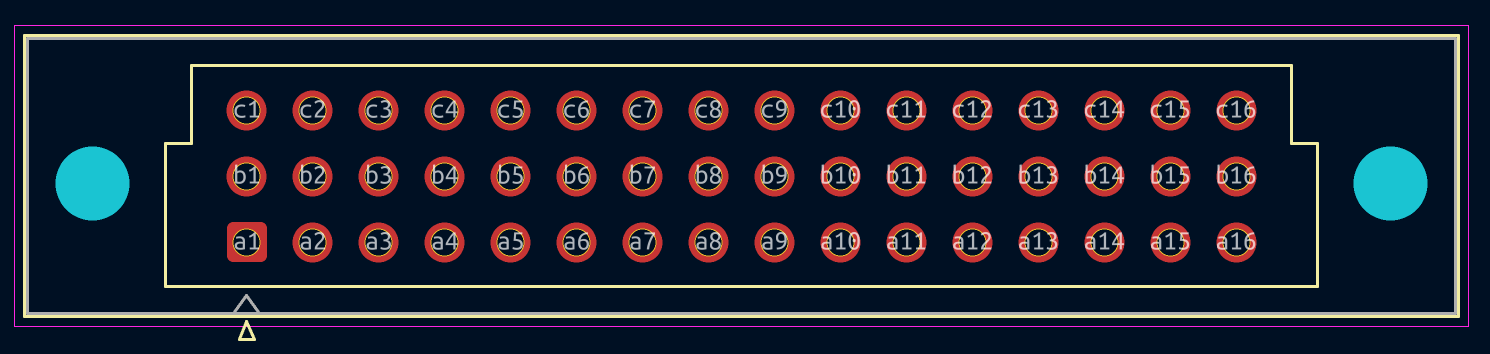
\includegraphics[width=0.5\textwidth]{photos/Footprint_Chainbus_altmode.png}
  \caption{DIN 41612 pinout}
  %\label{fig:NoLabel}
\end{figure}

\begin{table}[H]
  \centering
  \small
  \begin{tabular}{@{}llll@{}}
    \toprule
    \textbf{Pin \#} & \textbf{Row A (AltMode)} & \textbf{Row B (Address/Bus)} & \textbf{Row C (Power)} \\ \midrule
    1               & Altmode 1                & ADDR 1                       & GND                    \\
    2               & Altmode 2                & ADDR 2                       & +5V                    \\
    3               & Altmode 3                & ADDR 3                       & +5V                    \\
    4               & Altmode 4                & ADDR 4                       & GND                    \\
    5               & Altmode 5                & ADDR 5                       & BRD\_VIN               \\
    6               & Altmode 6                & ADDR 6                       & BRD\_VIN               \\
    7               & Altmode 7                & ADDR 7                       & BRD\_VIN               \\
    8               & Altmode 8                & ADDR 8                       & BRD\_VIN               \\
    9               & Altmode 9                & ChainBus SDA                 & GND                    \\
    10              & Altmode 10               & ChainBus SCL                 & GND                    \\
    11              & Altmode 11               & ChainBus CS                  & GND                    \\
    12              & Altmode 12               & ChainBus SCK                 & GND                    \\
    13              & Altmode 13               & ChainBus MOSI                & Reserved               \\
    14              & Altmode 14               & ChainBus MISO                & Reserved               \\
    15              & Altmode 15               & ChainBus RX                  & +12V stby              \\
    16              & Altmode 16               & ChainBus TX                  & GND                    \\ \bottomrule
  \end{tabular}
\end{table}

\subsection{ChainBus}
Jest na każdym hacie.

\begin{figure}[!ht]
  \centering
  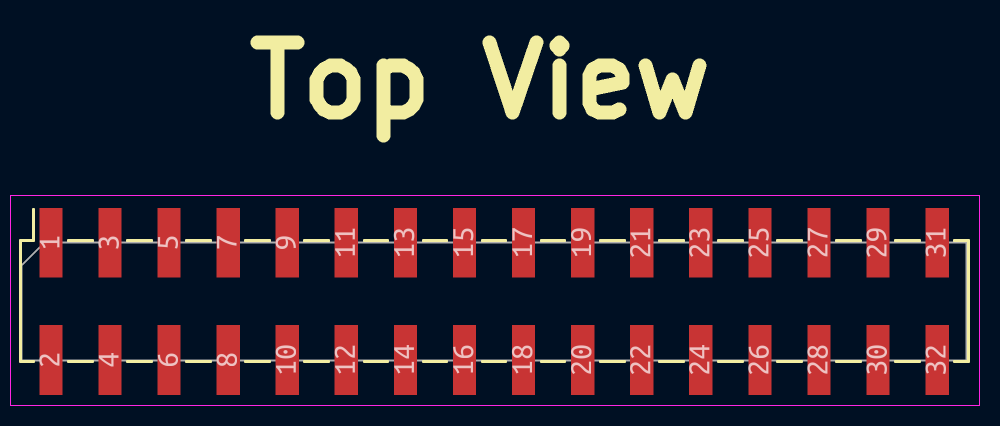
\includegraphics[width=0.5\textwidth]{photos/footprint_chainbus.png}
  \caption{Złącza 2x16 SMD na górnej warstwie}
  %\label{fig:NoLabel}
\end{figure}

Okay, wątek jest taki - ChainBus trzeba dać na górnej i dolnej warstwie. Wszystkie piny poza ADDR idą
bezpośrednio z dolnej do górnej, a ADDR idą z przeplotem.

\begin{table}[!ht]
  \centering
  \caption{ChainBus in, dolna warstwa, 2x16 smd male}
  \small
  \begin{tabular}{@{}cl|cl@{}}
    \toprule
    \textbf{Pin} & \textbf{Sygnał} & \textbf{Pin} & \textbf{Sygnał} \\ \midrule
    1            & GND             & 2            & ADDR1           \\
    3            & +5V             & 4            & ADDR2           \\
    5            & +5V             & 6            & ADDR3           \\
    7            & GND             & 8            & ADDR4           \\
    9            & VIN\_ChainBus   & 10           & ADDR5           \\
    11           & VIN\_ChainBus   & 12           & ADDR6           \\
    13           & VIN\_ChainBus   & 14           & ADDR7           \\
    15           & VIN\_ChainBus   & 16           & ADDR8           \\
    17           & GND             & 18           & ChainBus SDA    \\
    19           & GND             & 20           & ChainBus SCL    \\
    21           & GND             & 22           & ChainBus CS     \\
    23           & GND             & 24           & ChainBus SCK    \\
    25           & Reserved         & 26           & ChainBus MOSI   \\
    27           & Reserved         & 28           & ChainBus MISO   \\
    29           & +12V stby       & 30           & ChainBus TX     \\
    31           & GND             & 32           & ChainBus RX     \\ \bottomrule
  \end{tabular}
\end{table}

\begin{table}[H]
  \centering
  \caption{ChainBus out, górna warstwa, 2x16 smd female}
  \small
  \begin{tabular}{@{}cl|cl@{}}
    \toprule
    \textbf{Pin} & \textbf{Sygnał} & \textbf{Pin} & \textbf{Sygnał} \\ \midrule
    1            & GND             & 2            & ADDR2           \\
    3            & +5V             & 4            & ADDR3           \\
    5            & +5V             & 6            & ADDR4           \\
    7            & GND             & 8            & ADDR5           \\
    9            & VIN\_ChainBus   & 10           & ADDR6           \\
    11           & VIN\_ChainBus   & 12           & ADDR7           \\
    13           & VIN\_ChainBus   & 14           & ADDR8           \\
    15           & VIN\_ChainBus   & 16           & NC              \\
    17           & GND             & 18           & ChainBus SDA    \\
    19           & GND             & 20           & ChainBus SCL    \\
    21           & GND             & 22           & ChainBus CS     \\
    23           & GND             & 24           & ChainBus SCK    \\
    25           & Reserved         & 26           & ChainBus MOSI   \\
    27           & Reserved        & 28           & ChainBus MISO   \\
    29           & +12V stby       & 30           & ChainBus TX     \\
    31           & GND             & 32           & ChainBus RX     \\ \bottomrule
  \end{tabular}
\end{table}

No, ale z TX RX uważaj (;

\subsection{ChainLink}
2x są na każdym MMS3 i są na kartach adapter.

\begin{figure}[H]
  \centering
  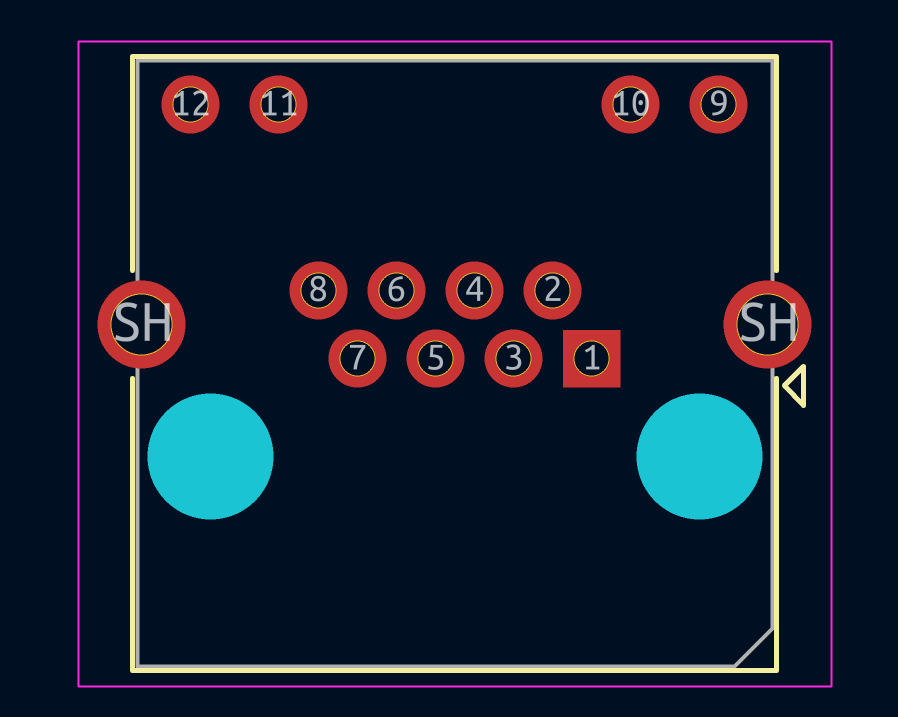
\includegraphics[width=0.5\textwidth]{photos/footprint_rj45.png}
  \caption{Złącze RJ45}
  %\label{fig:NoLabel}
\end{figure}

\begin{table}[H]
  \centering
  \begin{tabular}{@{}cll@{}}
    \toprule
    \textbf{Pin} & \textbf{Sygnał} \\ \midrule
    1            & CAN1.-          \\
    2            & CAN1.+          \\
    3            & GND             \\
    4            & CAN2.-          \\
    5            & CAN2.+          \\
    6            & +12V stby       \\
    7            & USB\_MMS\_.D-   \\
    8            & USB\_MMS\_.D+   \\ \bottomrule
  \end{tabular}
\end{table}

\subsection{XT60}
Zasilanie, pewnie wszędzie jest.

\begin{figure}[H]
  \centering
  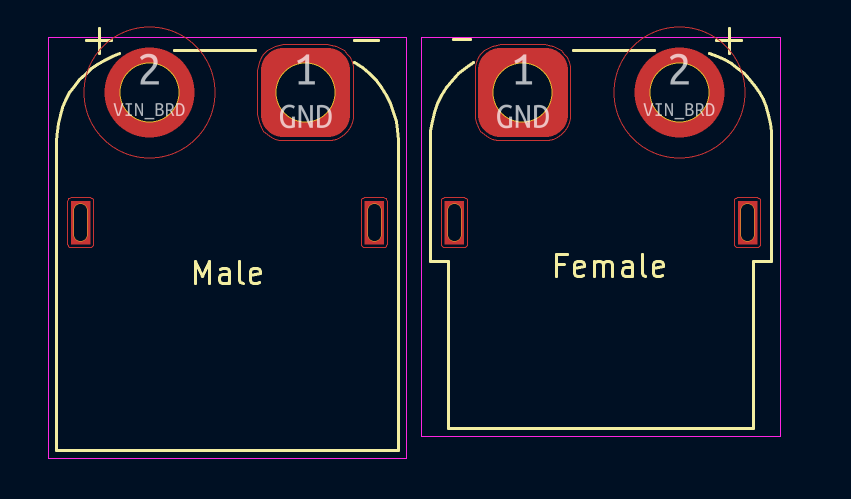
\includegraphics[width=0.5\textwidth]{photos/footprint_XT60.png}
  \caption{XT60 męska i żeńska}
  %\label{fig:NoLabel}
\end{figure}

\subsection{JST-XH}
Wszystko idzie na JST-XH z rastrem 2.54 (same as goldpin), więc nie można dać uniwersalnego pinoutu.

Jedynie powiem, że preferowany jest GND na pinie 1.

\subsection{I2C}
Jak masz I2C na hatach, to to jest preferowany pinout:

\begin{figure}[H]
  \centering
  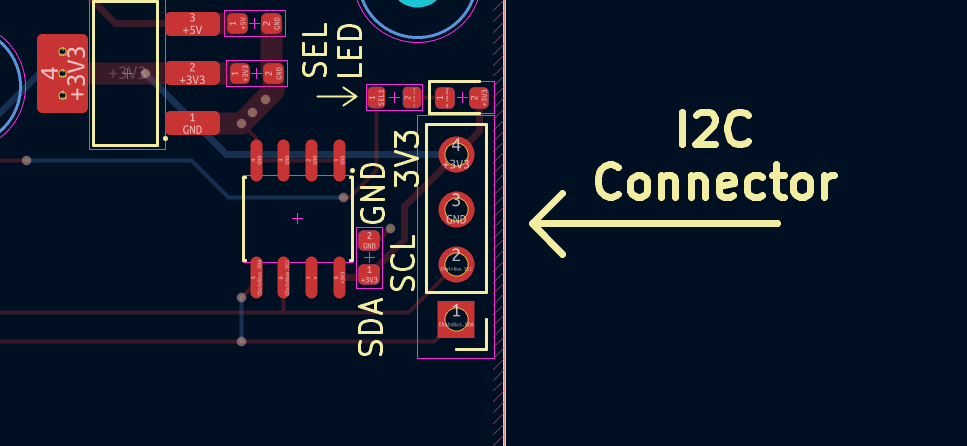
\includegraphics[width=0.5\textwidth]{photos/footprint_I2C.png}
  \caption{Złącze goldpin 1x4 z I2C na nim}
  %\label{fig:NoLabel}
\end{figure}

\subsection{Programowanie MCU na hatach}
Jeśli masz MCU na hacie, to to są preferowane pinouty złącz do flashowania:

\subsubsection{CH32V003}
Jest podobne do WCH Link-E.

\begin{figure}[H]
  \centering
  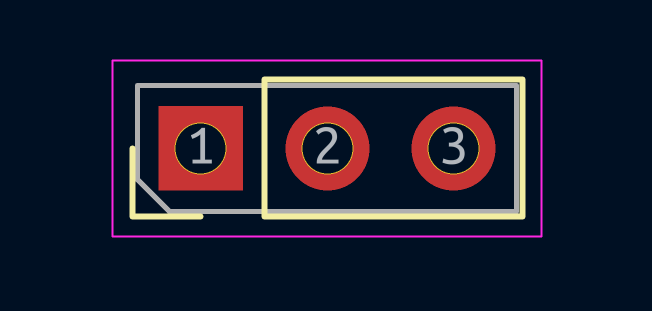
\includegraphics[width=0.5\textwidth]{photos/footprint_jst_xh_3pin.png}
  \caption{JST-XH 1x3}
  %\label{fig:NoLabel}
\end{figure}

\begin{table}[H]
  \centering
  \begin{tabular}{@{}cll@{}}
    \toprule
    \textbf{Pin} & \textbf{Sygnał} \\ \midrule
    1            & SWIO            \\
    2            & GND             \\
    3            & 3V3             \\
  \end{tabular}
\end{table}



\section{Duży ModuCard - Zasada działania}
\subsection{Overview}
Bazą dużego ModuCard'a jest backplane - duża płytka pcb z ze złaczami na karty. Do niego wpina się karty ModuCard. System podobny do Eurocard'a albo PCI w komputerach.

Do kart jest podłączone 2xCan, USB i pare innych rzeczy

Dalej, karty. Na nich jest cała faktyczna elektronika którą potrzebuesz - mikroprocesory, czujniki, komputery, zasilacze etc. Każda karta to kompletny system ze swoim MCU i wszystkim.

Są 3x typy kart

1. Karta komputer pokładowy -> Np. Rasperry Pi 5 czy jakiś minikomputer Jetson. Do niego raportuje reszta kart, on przetważa te dane i zwraca kartą co mają robić

2. Karta zasilacz -> przejściówka z baterii lub 230V na +48V które zasila cały system

3. Karta użytkowa -> Normalna karta która coś robi, np. Karta Nawigacji, Karta przekaźników etc

Dla kompletnego systemu potrzebujesz 1x Karte komputera pokładowego. 1 lub więcej Karte zasilacza i ile ci się zmieści kart użytkowych 

\subsubsection{I ważne, Duży moducard można seamless podłączyć z MMS -> \ref{karta_adapter}}
\subsubsection{Oh, i to może cie też interesować}
Kiedy którego użyć -> \ref{Kiedy_ktorego_uzyc}

\section{Duży ModuCard - Backplane}
Szkielet całego ModuCard'a -> do niego wpinasz karty

% /#\#/\/#\ Zdjęcie pliska

Backplane przekazuje między kartami
\begin{itemize}
  \item 2x CAN
  \item 1x USB na karte. podłączone do komputera pokładowego
  \item 2x Strobe (o nich w \ref{Duży ModuCard - Strobe})
  \item 16x GPIO (o nich w \ref{Duży ModuCard -  GPIO})
  \item Zasilanie 48V (ile mocy/karte masz w \ref{Duży ModuCard - Bilans Mocy})
  \item I troche pinów konfiguracyjnych
\end{itemize}

USB jest podłączone przez hub'a USB wbudowanego w backplane'a.

Na całego backplane'a możesz dać tylko jeden komputer pokładowy, musi być w slot'ie pierwszym.

Backplane'y można łączyć ze sobą żeby je przedłużyć. Np. dwa backplane'y 6x można połączyć w jednego 12x. Oh i pamiętaj że komputer pokładowy musi być w slot'ie pierwszym pierwszego backplane'a

Co do pinów konfiguracyjnych, to don't worry about them (:

% /#\#/\/#\ Jak będziemy mieli piny konfiguracyjne to je opisze (;

\section{Duży ModuCard - Typy Kart}
\subsection{Karta Gateway (Komputer pokładowy)}
Pierwsza i najważniejsza karta w systemie. To ona steruje wszystkim.

Jest na niej minikomputer, Np. raspberry Pi, Nvidia Jetson czy to tam potrzebujesz. On rozmawia z kartami po USB i CAN, przetważa te dane i wysyła kartą co mają robić. Pewnie jest na nim ROS (Robotic Operating System)

Możesz go zaprogramować jako
1. Komputer pokładowy - no, komputer pokładowy. Niezależna jednostka która steruje całym robotem.
2. Gateway - Jeśli potrzebujesz mega dużo mocy obliczeniowej to zamiast robić jakiś porąbanie mocny komputer pokładowy i przetważać te dane w robocie, to wysyłasz dane po np. Ethernecie poza robota, tam to przetważasz i odsyłasz spowrotem do robota. Wtedy karta komputera pokładowego robi jako gateway do innego, większego komputera

Wymiennie będę nazywał tą karte jako komputer pokładowy i gateway.

\subsection{Karta Zasilacza}
Dostaje zewnętrzne zasilanie i przetwarza je na zasilanie +48V na głównej szynie zasilania moducarda i co tam potrzeba. Możesz go zrobić żeby dostawał zasialnie z baterii jak nomad, z zasilacza ATX jak Hefajstos czy z 230V.

Obsługuje (as in: powinna obsługiwać) sekwencjonowanie zasilania czyli odpalanie po kolei poszczegółnych szyn i raportowanie ich stanu do komputera pokładowego

Jaką chcemy sekwencje mieć, to trzeba jeszcze wymyślić albo ukraść z MMS2

\subsection{Karta użytkowa}
I karta najbliższa twojemu sercu (chyba że jesteś programistą ROS'a) czyli karta użytkowa.

Na karcie użytkowej implementujesz to co potrzebujesz - IC do GPS, enkodera, przekaźniki whatever. Do tego jakieś MCU i na piwo

MCU jest podłączone przez Backplane'a do Komputera pokładowego. Raportuje mu tam co i jak.

No i tyle. cała sztuka. To jest basic bitch embedded system, tylko na standardowym PCB i ma CAN'a.

No i ofc potrzebujesz przetworki 48V -> 5V or whatever floats your boat.


\section{Do czego używać GPIO L/R} \label{Duży ModuCard -  GPIO}
Każda karta ma 16 GPIO wyprowadzonych do komunikowania się z kartami obok. Możesz ich używać do
\begin{itemize}
  \item Do niczego - Najlepsza opcja, każda karta jest niezależna i może ją wpiąć gdzie chcesz i się nie martwić o nic. Jeśli możesz to tak zrób
  \item Jeśli jakoś absolutnie brakuje ci miejsca na PCB i nie możesz tego rozbić na niezależne karty, to możesz podzielić to co robisz na dwie karty które komunikują się czy to cyfrowo czy analogowo czy jakieś interrupty przez GPIO L/R. Jak możesz to zrób dwie niezależne karty, i dopiero jak się tak nie da to zrób z komunikacją przez GPIO.
  \item Jest 16 GPIO, i wiesz co ma też 16 GPIO? Chainbus. Możesz zrobić system MMS na dużym ModuCard'ie. Ale no, lepiej robić niezależne karty
  \item Tak na prawde miedź to miedź, więc możesz na nich cokolwiek puścić. Use your own judgment and creativity
\end{itemize}

Long story short, nie przejmuj się nim
\section{Co to strobe} \label{Duży ModuCard - Strobe}
Strobe to para różnicowa do timingu. Gdybyś potrzebował dokładnie zsynchronizować jakieś wydarzenie na hat'ach to możesz wysłać na to trigger. Nigdzie tego jeszcze nie potrzebowaliśmy, jest jako futureproofing.

Long story short, nie przejmuj się nim
\section{Duży ModuCard - Przykładowe Karty}
\section{Duży ModuCard - Bilans Mocy}\label{Duży ModuCard - Bilans Mocy}
\section{Duży ModuCard - Wymagania dla Kart użytkowych}
\section{Duży ModuCard - Wymagania dla Kart zasilacza}
\section{Duży ModuCard - Wymagania dla Kart komputera pokładowego}
\section{Duży ModuCard - Wymagania dla Backplane'a}
\section{Duży ModuCard - Projektowanie kart} \label{Duży ModuCard - Projektowanie kart}
Sorka, To be done
\section{Duży ModuCard - Pinout złączy}

\section{Pomiędzy systemami - Karta adapter i ChainLink} \label{karta_adapter}
\subsection{Karta Adapter}
Przez Backplane ModuCard'a głównym protokołem komunikacji jest CAN. To na nim hat'y wysyłają informacje do Komputera pokładowego.

Karta adapter bierze tego CAN'a oraz USB i wystawia je na złączke RJ45 (ta sama co ethernet jest). I teraz, do tego możesz podłączyć MMS3.

I to jest tak, że MMS3 ma dostęp do całej komunikacji jakie mają karty na Backplane'ie.

Tego Can'a, USB (i +12V) na RJ45 nazywamy ChainLink. Oh, i chyba pinoutowo to jest kompatybilne albo z VESC albo z BetaFlight

I jeszcze karta adapter może sekwencjonować zasilanie MMS3. Czyli po kolei włączać kolejne wiązki i sprawdzać czy gdzieś jest zwaracie zasilania, ale to TBD jest.

\subsection{Łączenie systemów}
Okay, gadamy sobie o dwóch różnych systemach - MiniModuCard i ModuCard. Ale one podobno są "połączone" ze sobą. Trik jest taki

Karta komputera pokładowego steruje całym systemem. Tak na prawde jeśli coś może do niej gadać, to jest kompatybilne z ModuCard'em.

Karty, proste - gadają z nią po CAN'ie i USB przez Backplane'a

Teraz MMS, on jest podłączony po CAN'ie, przez karte adapter do Komputera . Z punktu widzenia komputera nie ma różnicy czy coś jest mówi do niego MMS3 czy jakaś Karta, komunikacja jest taka sama

I to tyle.

Jeszcze inny trik jest taki staram się dawać takie same MCU (STM32F305) i na karty, i na MMS3 więc programować się je będzie tak samo. Łatwo będzie przeportować stack can'a z jednego na drugie oraz jak zaprogramujesz jedno to od razu potrafisz drugie.

\section{Pomiędzy systemami - Duży moducard a mały, kiedy którego użyć} \label{Kiedy_ktorego_uzyc}
Możesz mieć pytanie "Ej, te dwa systemy to praktycznie to samo" albo "Musze zrobić XXX, to potrzebuje dużego czy małego moducard". Ja o tym tak myśle

% /#\#/\/#\ Tutaj coś dopisze jak zrobie pare kart i zobacze z czym to się je

Mały task - mały moducard. Duży task - moducard nie musi być duży, ale tak się łatwiej projektuje
% Mały rysunek, mała wiedza. Duży rysunek - więdza może i nie jest duża, ale przynajmniej jest czytelnie - Jacek Świniarski, mój ulubiony zawodowiec z technikum

\chapter{Książka programisty}
\section{Wstęp}
Aktualnie nie mamy nic zaprogramowane. Powodzenia!

Update: Chyba używamy Zephyr'a
\chapter{Książka mechaniczna}
\section{Gotowe rozwiązania}
Siemka, jak nie chce ci się projektować, to możesz zakosić jeden z tych sposobów na który już mocowaliśmy ModuCard'a
\subsection{MMS -> Szyna DIN}
To Do
% /#\#/\/#\ To Do
\subsection{ModuCard -> Bojowe zadanie}
Jest 60\% szansy że ModuCard jest natywnie kompatybilny z EuroCard'em. Weź sprawdź czy faktycznie jest i mi napisz pliska <3
\subsection{ModuCard -> Nic nie ma jeszcze}
W sensie nomad coś montował, ale tbh nie wiem. Oni mieli jeszcze ModuCard2 a tu gadamy o ModuCard3, ale powinno być kompatybilne\dots

\section{Wymiary}
Najlepszą metodą na złapanie wymiarów jest poproszenie elektronika, żeby wyeksportował ci PCB do .step razem z komponentami i wbicie tego do twojego CAD'a

Ta sekcja jest bardziej pod kątem utrzymania standardu.

Wymiary do śrub montażowych albo keepout zone'ów (to jest miejsce, gdzie elektronik nie może stawiać komponentów i ty możesz tam sobie coś zamodelować do zamocowania hata) - są symetryczne, więc paru wymiarów nie podałem.


\subsection{Duży ModuCard}
To Do
\subsection{MiniModuCard - MMS3 (Mikrokontroler)}
To Do
\subsection{MiniModuCard - Hat}
Odległość między hatem a hatem albo MMS3 a hatem to 1 złącze goldpin SMD męskie + wpięte w nie SMD żeńskie. To chyba jakieś 25.4 mm czy tam 1 cal ale weź to jeszcze sprawdź bo z głowy to pisze.
\begin{figure}[!h]
  \centering
  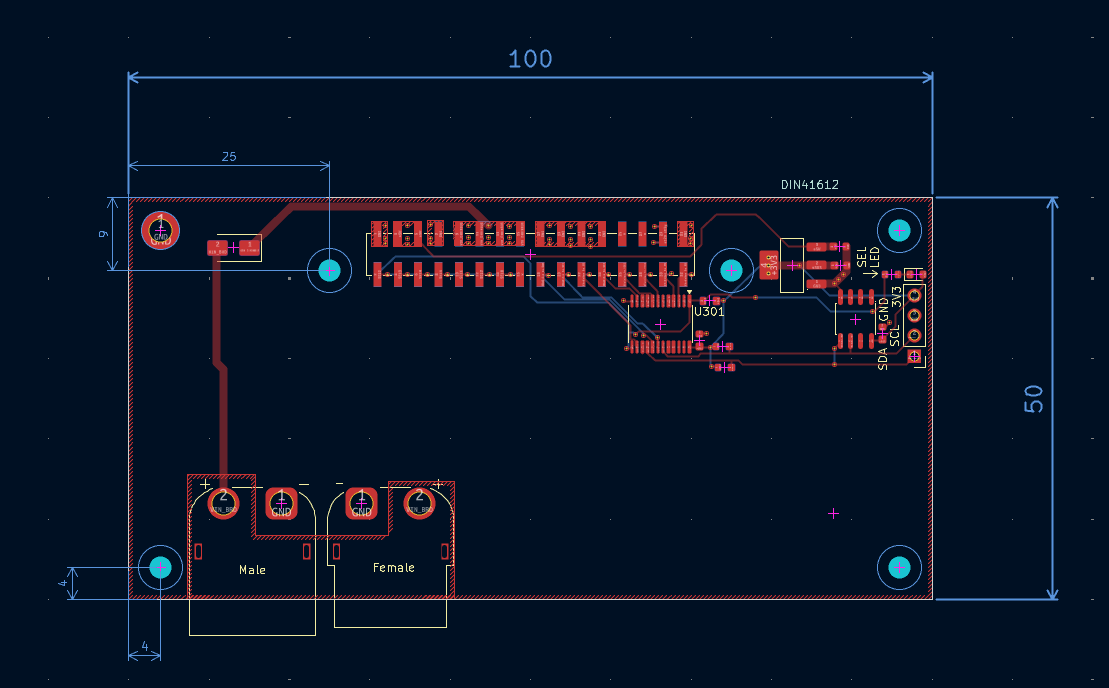
\includegraphics[width=0.8\textwidth]{photos/MMS_Hat_Dimensions_1.png}
  \caption{Wymiary płytki i otworów montażowych}
  %\label{fig:NoLabel}
\end{figure}


\begin{figure}[!h]
  \centering
  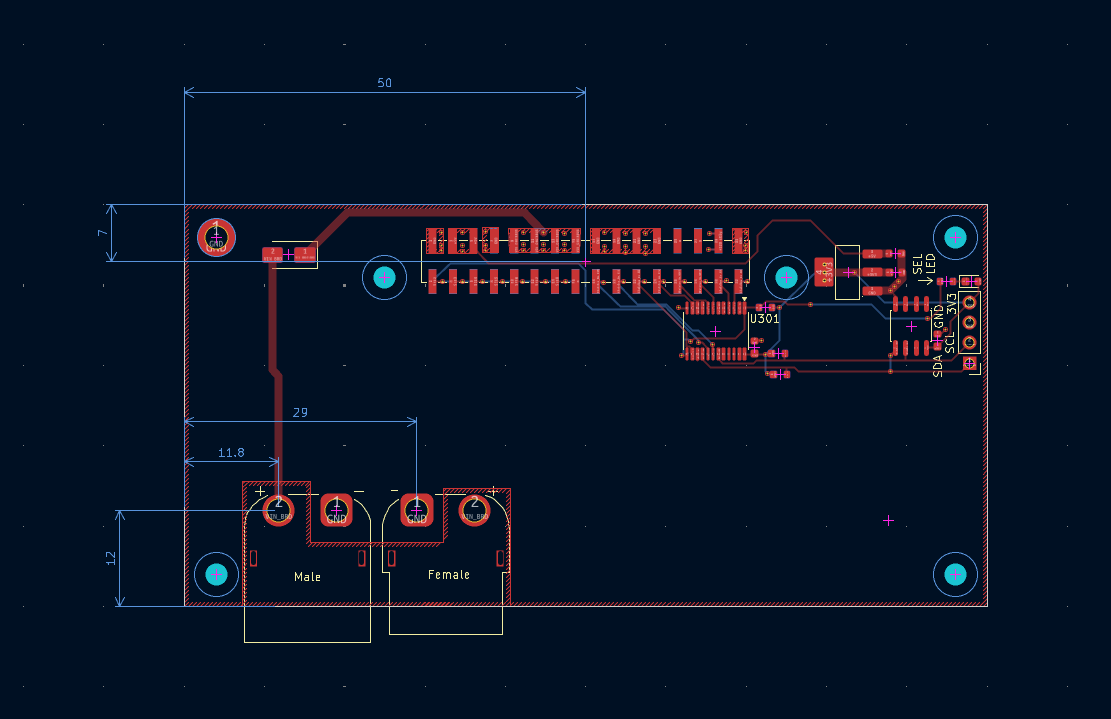
\includegraphics[width=0.8\textwidth]{photos/MMS_Hat_Dimensions_2.png}
  \caption{Rozstaw złącz}
  %\label{fig:NoLabel}
\end{figure}

Te złącza w lewym dolnym to XT60 i tbh nie muszą być co do milimetra w tym miejscu.
Ważne, żeby były jak najbardziej w lewym dolnym i pierwsze męskie, a potem żeńskie.


\begin{figure}[!h]
  \centering
  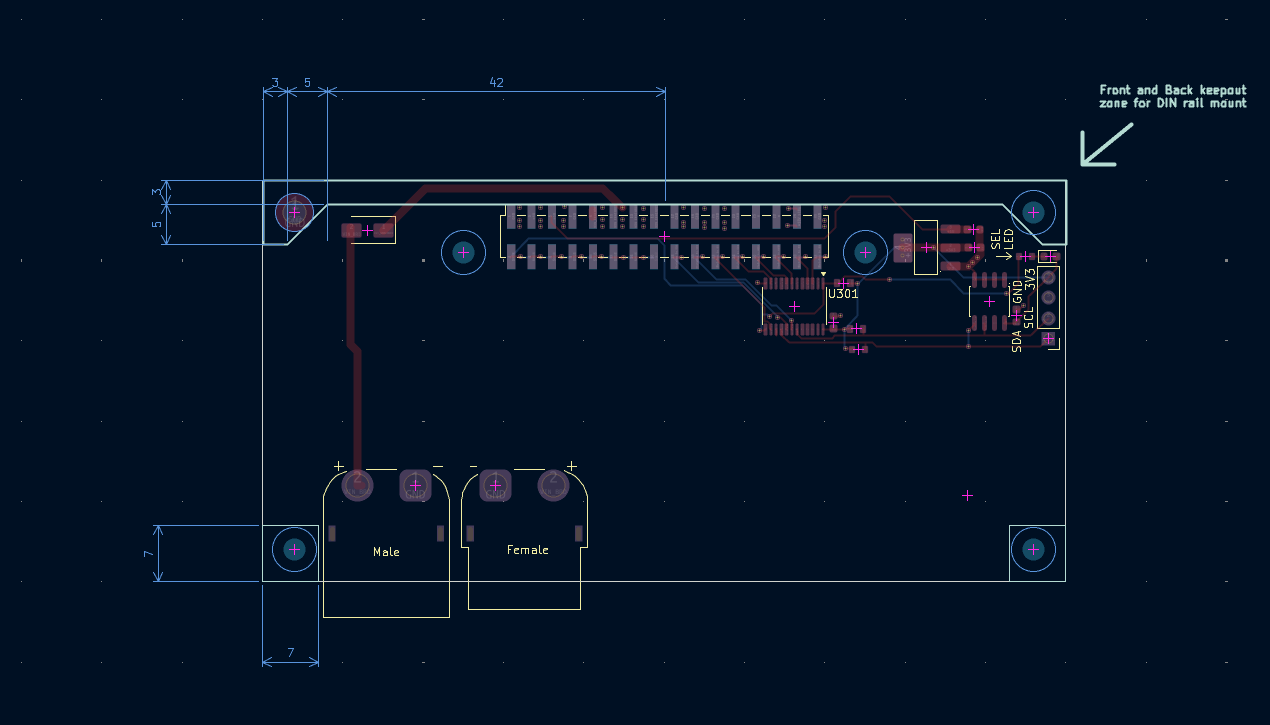
\includegraphics[width=0.8\textwidth]{photos/MMS_Hat_Dimensions_3.png}
  \caption{Miejsce zarezerwowane na montaż}
  %\label{fig:NoLabel}
\end{figure}

\chapter{Książka system integrator}
\chapter{Książka ecosystem maintainer}

Okay, jako że to jest mój fork to sobie zapisze notatki co do rozwoju systemu

\begin{itemize}
  \item Nazwa MMS3 both do systemu Kontroler + hat i też do samego controlera jest confusing
  \item trzeba wymyślić nazwe na hat'y który 1. nie zabierają ADDR 2. Odwalaja coś z ADDR (hat PSU i hat hat expander)
  \item każdy projekt na githubie musi mieć tag żeby dało rade go szukać sensownie
  \item programowanie musi być proste, KISS it or nobody will use it
  \item Trzeba porządnie usiąść do licencji prawnych. Hat'y mają jakieś, ale to temp solutions
  \item Czy da rade zrobić interrupty na ChainBus? Pomysł jest taki: ADDRX pullup i hat może go sam pulnąć w dół jak coś się dzieje - zły pomysł
\end{itemize}


\end{document}


% Możesz szukać tego
% /#\#/\/#\ 